\documentclass[color=usenames,dvipsnames]{beamer}
%\documentclass[color=usenames,dvipsnames,handout]{beamer}

%\usepackage[roman]{../pres1}
\usepackage[sans]{../pres1}
%\usepackage{pdfpages}
\usepackage{animate}
\usepackage{pgfpages}
\usepackage{xmpmulti}

%\setbeameroption{notes on second screen}
%\renewcommand*\sfdefault{lmss} % cmss, lmss (latin modern), phv (Helvetica) qhv, qag
%\renewcommand*\rmdefault{ptm} %



\begin{document}


%\setlength{\fboxsep}{0pt}


\begin{frame}[plain]
  \begin{center}
    {\LARGE {Applied Population Dynamics} \\
     \Large WILD 5700/7700 \\ 
     % \large January 7, 2019} \par
     \large
     Richard Chandler \\ }
   \vspace{3mm}
   \rule[0pt]{\textwidth}{0.1pt}
   \vspace{3mm}
  \end{center}

  {\setlength{\fboxsep}{0pt}
  \fbox{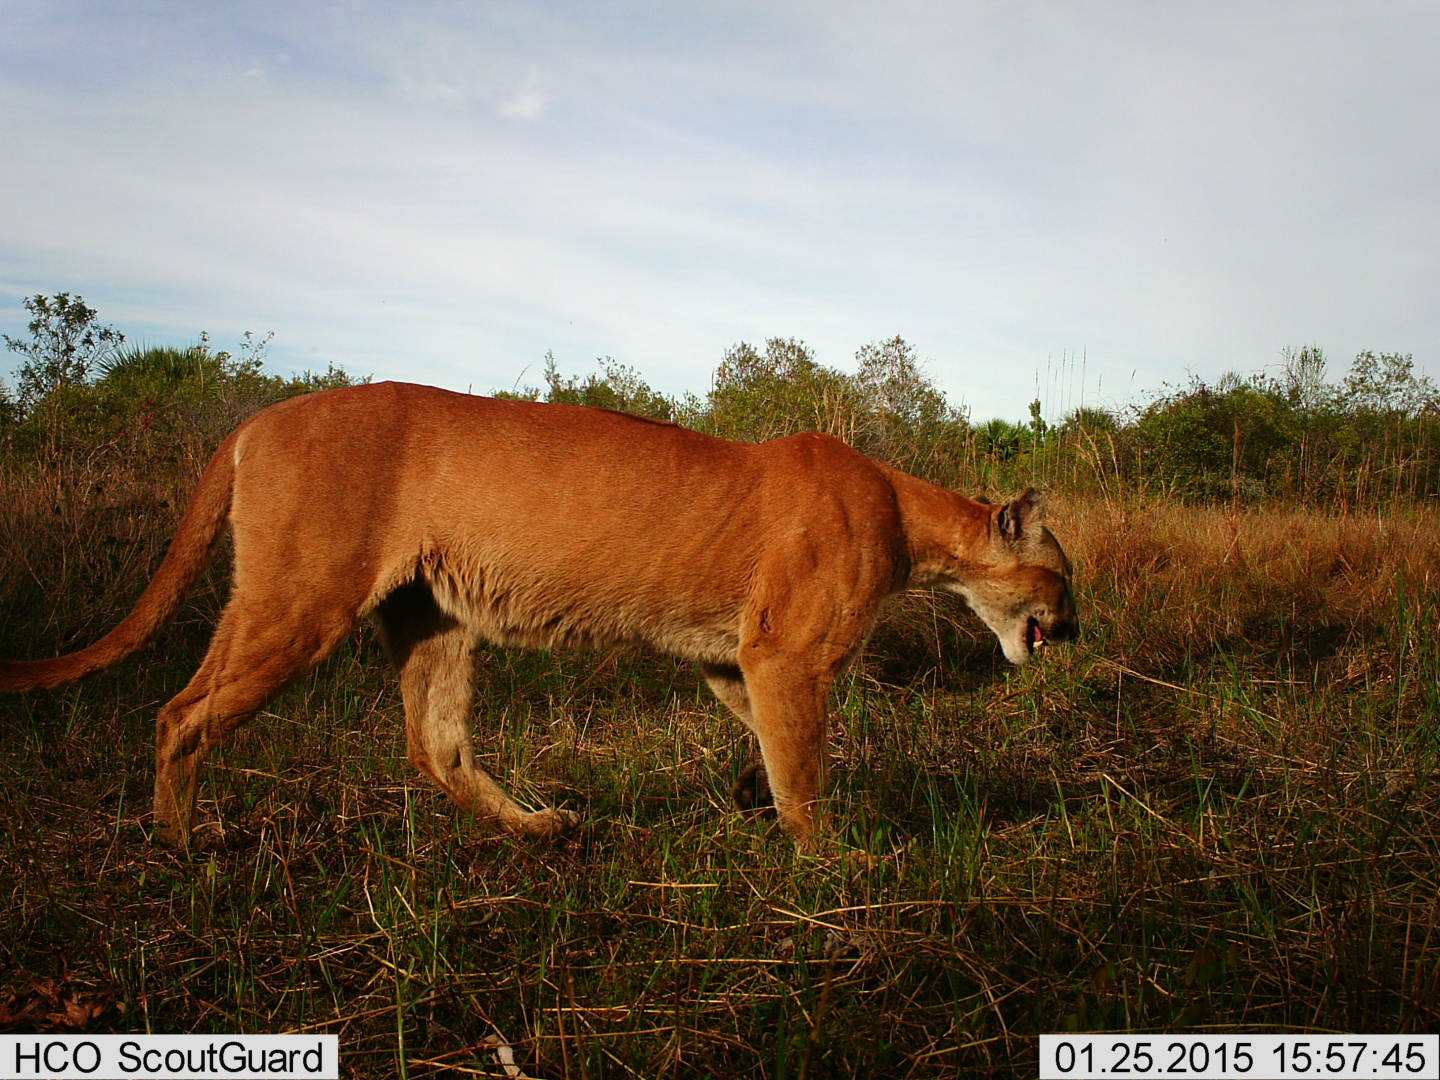
\includegraphics[height=3.9cm,keepaspectratio]{figs/puma1}} \hfill
  \fbox{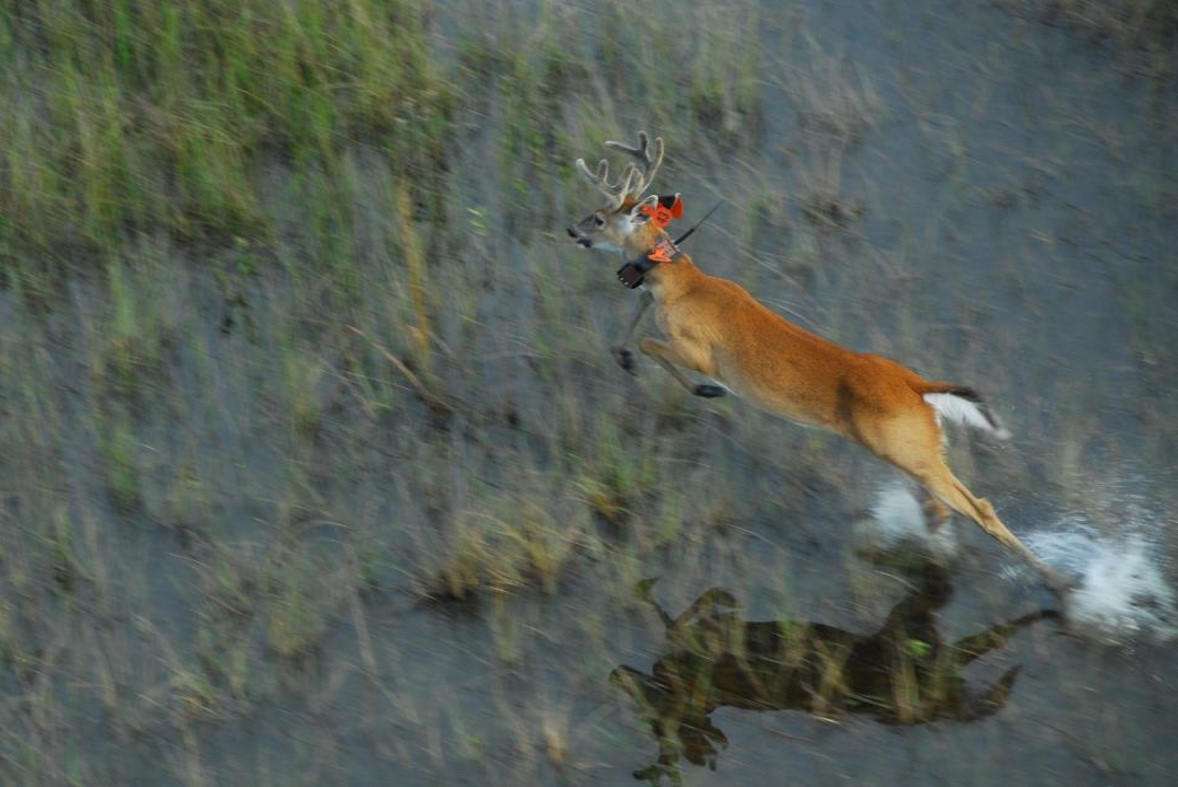
\includegraphics[height=3.9cm,keepaspectratio]{figs/deer_marked_helicopter}}
  }
  \note{Break down the title. Application and theory}
\end{frame}




\section{Introduction}


\begin{frame}
\frametitle{Central Questions}
  \large \centering
  \begin{enumerate}[\bf 1.]
    \item What causes spatial and temporal variation in population size
    and structure? \par
    \item[]
    \item<2-> How do environmental change and human activities (including
      management actions) affect populations?
  \end{enumerate}
\end{frame}



\begin{frame}
  \frametitle{Learning objectives}
  \large
  {\bf By the end of the semester, you should be able to: \\}
  \vspace{0.3cm}
  \begin{enumerate}[\bf 1.]
    \large
    \item<1-> Develop a population model that
      \begin{itemize}
        \normalsize %\large
        \item Describes variation in demographic parameters over time
        \item Predicts how a population will respond to
          management/conservation actions
      \end{itemize}
    \item[]
    \item<2-> Design a study to collect the data necessary to estimate
      the demographic parameters of the model
    \item[]
    \item<3-> Use software (e.g., {\tt R}, %{\tt PRESENCE}, {\tt DISTANCE},
      {\tt MARK}) to estimate parameters from field data
  \end{enumerate}
  \note{If you can do these three things well, you will do well as a
    wildlife ecologist}
\end{frame}



\begin{frame}
  \frametitle{Themes}
  \large
  \begin{itemize}
    \item[] {\hspace{-0.9cm} \bf Theory}
    \item Population models
    \item[]
    \item[] {\hspace{-0.9cm} \bf Practice (Application)}
    \item Study design
    \item Data collection
    \item Parameter estimation
    \item Harvest management
    \item Small population management
    \item Population viability analysis
  \end{itemize}
\end{frame}



\section{Examples}




\begin{frame}
  \frametitle{Example I -- Louisiana black bear}
  \begin{columns}
    \begin{column}{0.5\textwidth}
      \fbox{\includegraphics[width=\textwidth]{figs/laBear2}}
    \end{column}
    \begin{column}{0.5\textwidth}
      \fbox{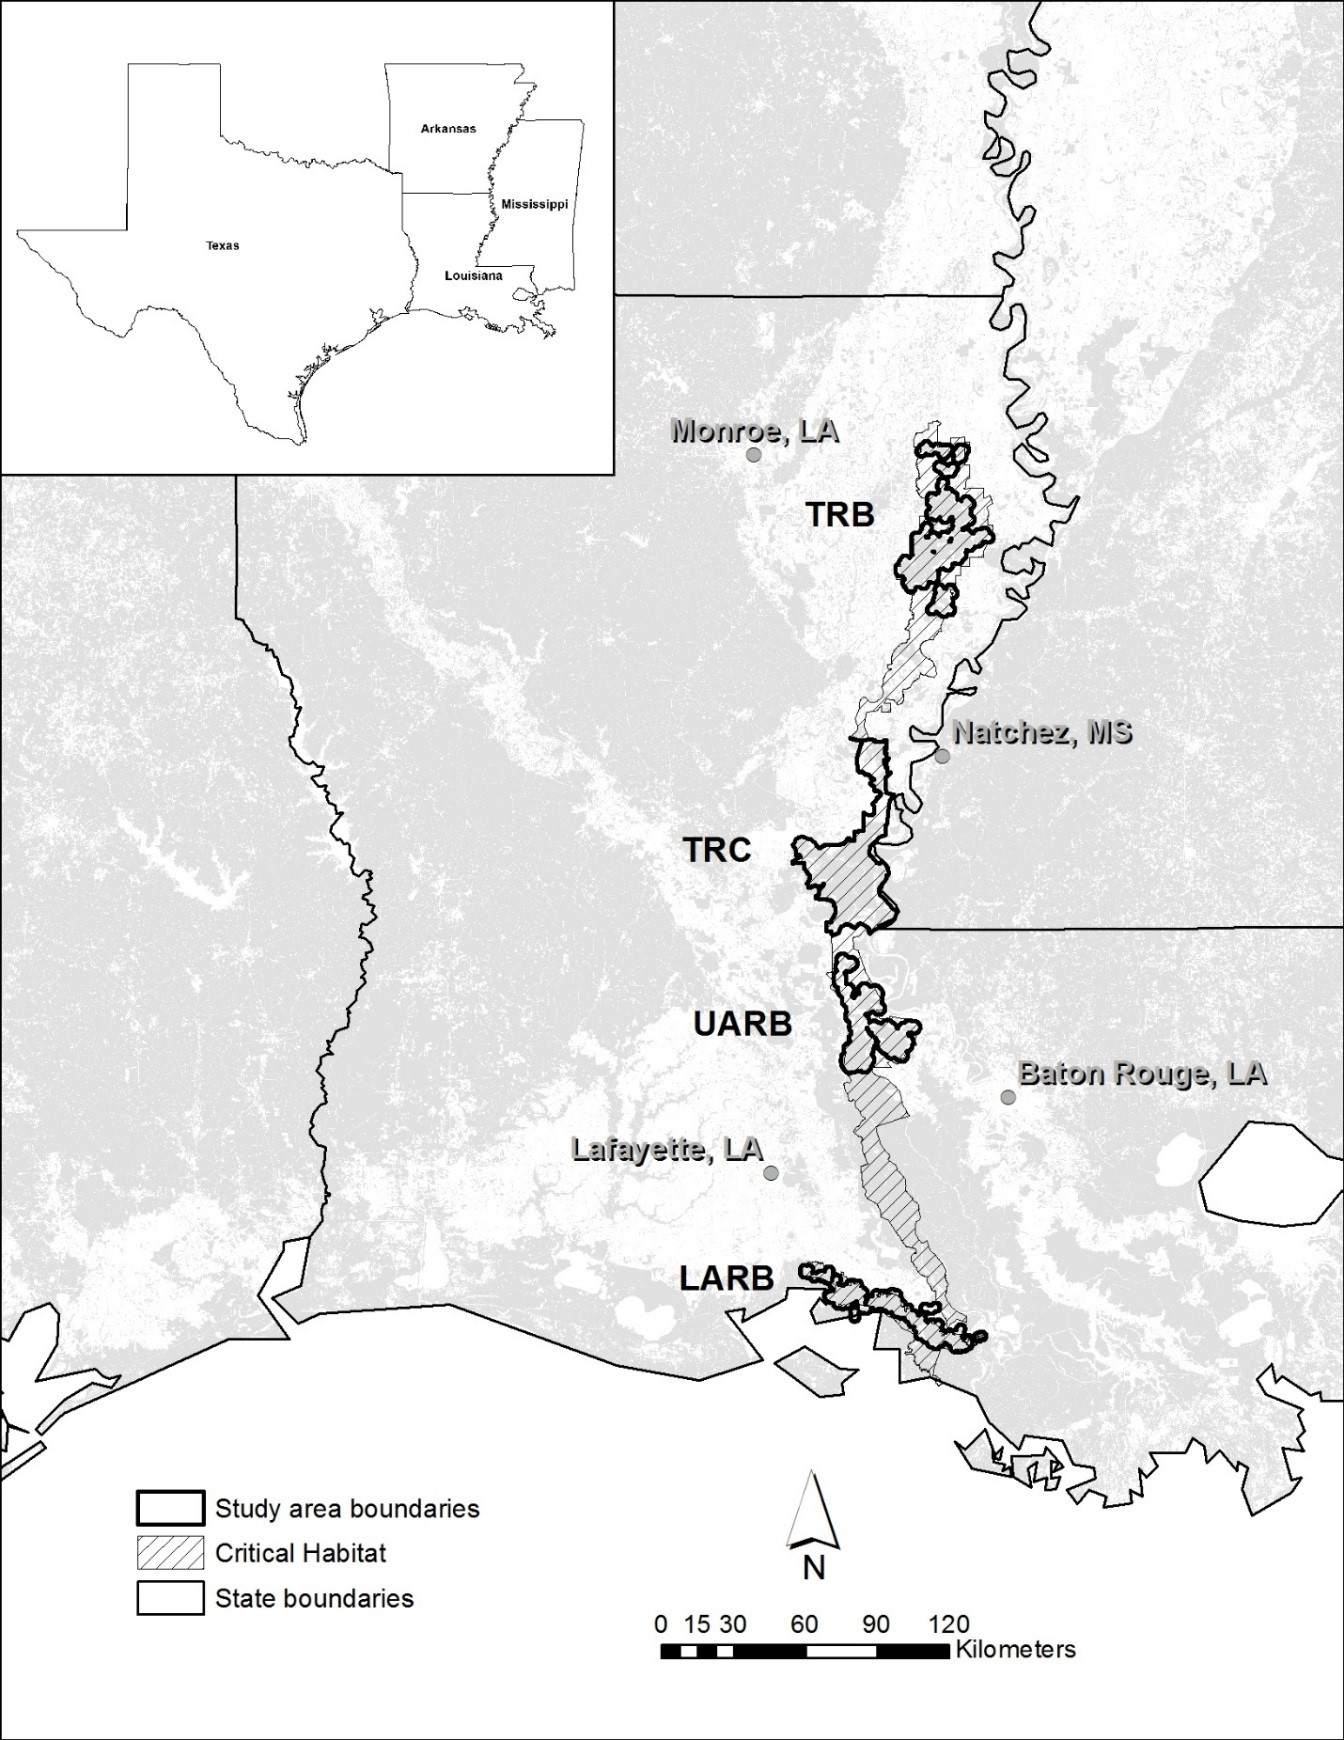
\includegraphics[width=\textwidth]{figs/LA-bear-map}}
    \end{column}
  \end{columns}
\end{frame}


\begin{frame}
  \frametitle{Estimated demographic parameters}
  \begin{center}
    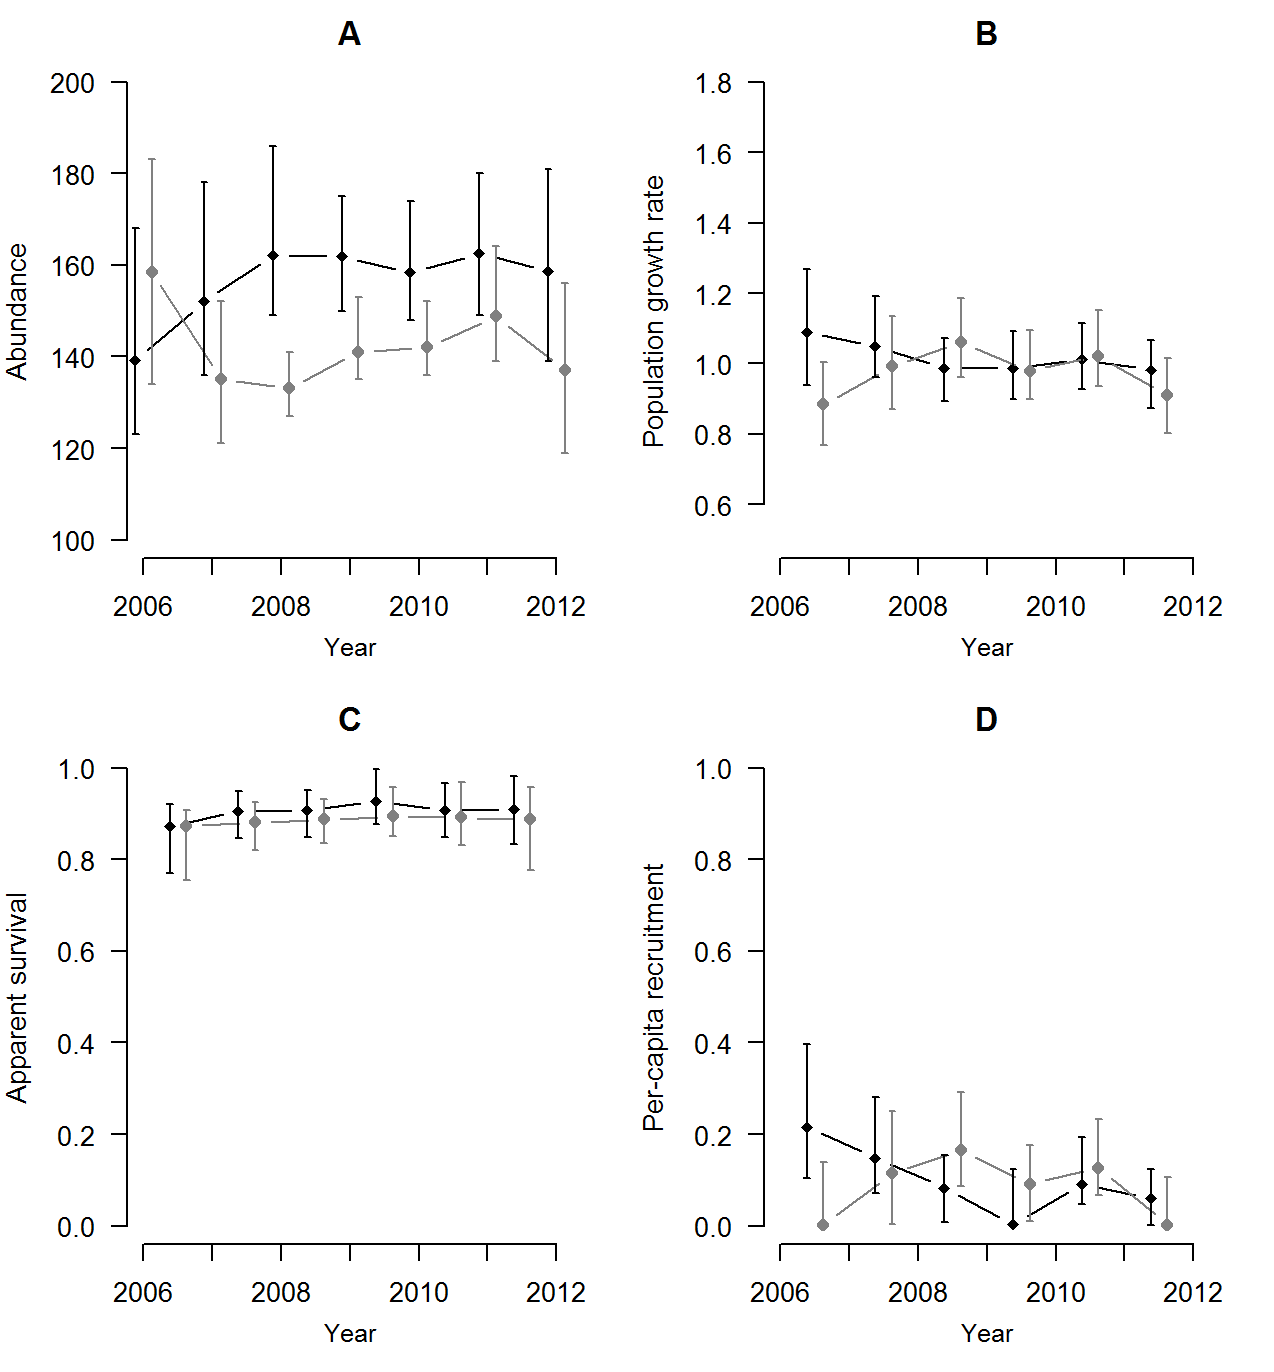
\includegraphics[width=0.7\textwidth]{figs/LA-bear-demographics}
  \end{center}
\end{frame}



\begin{frame}[fragile]
  \frametitle{Example II -- Black-throated blue warbler}
  {\centering
    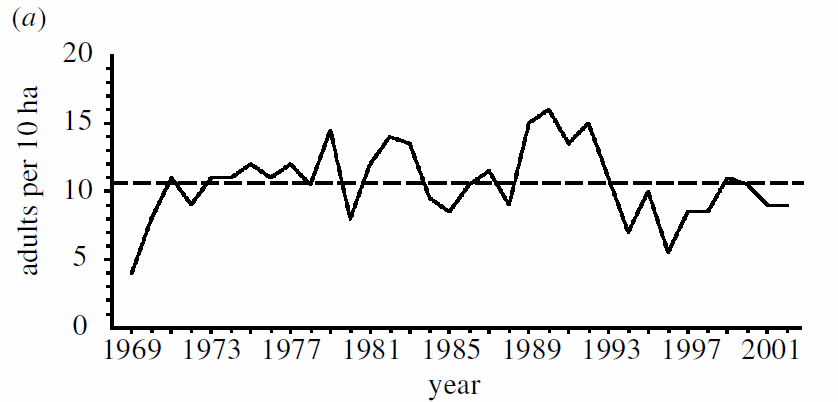
\includegraphics[width=0.9\textwidth]{figs/btbw}\let\thefootnote\relax\footnote{\tiny Rodenhouse et
      al. (2003, Proceedings of the Royle Society)} \\
  }
  \begin{columns}
    \begin{column}{0.8\textwidth}
    \end{column}
    \hfill
    \begin{column}{0.19\textwidth}
    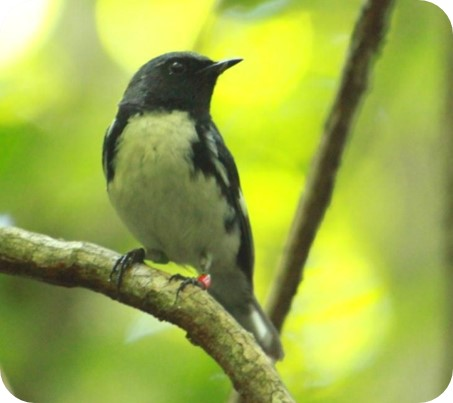
\includegraphics[width=\textwidth]{figs/btbw1}
  \end{column}
\end{columns}
\end{frame}




\begin{frame}[fragile]
  \frametitle{Example II -- Black-throated blue warbler}
  \centering \small %\large
  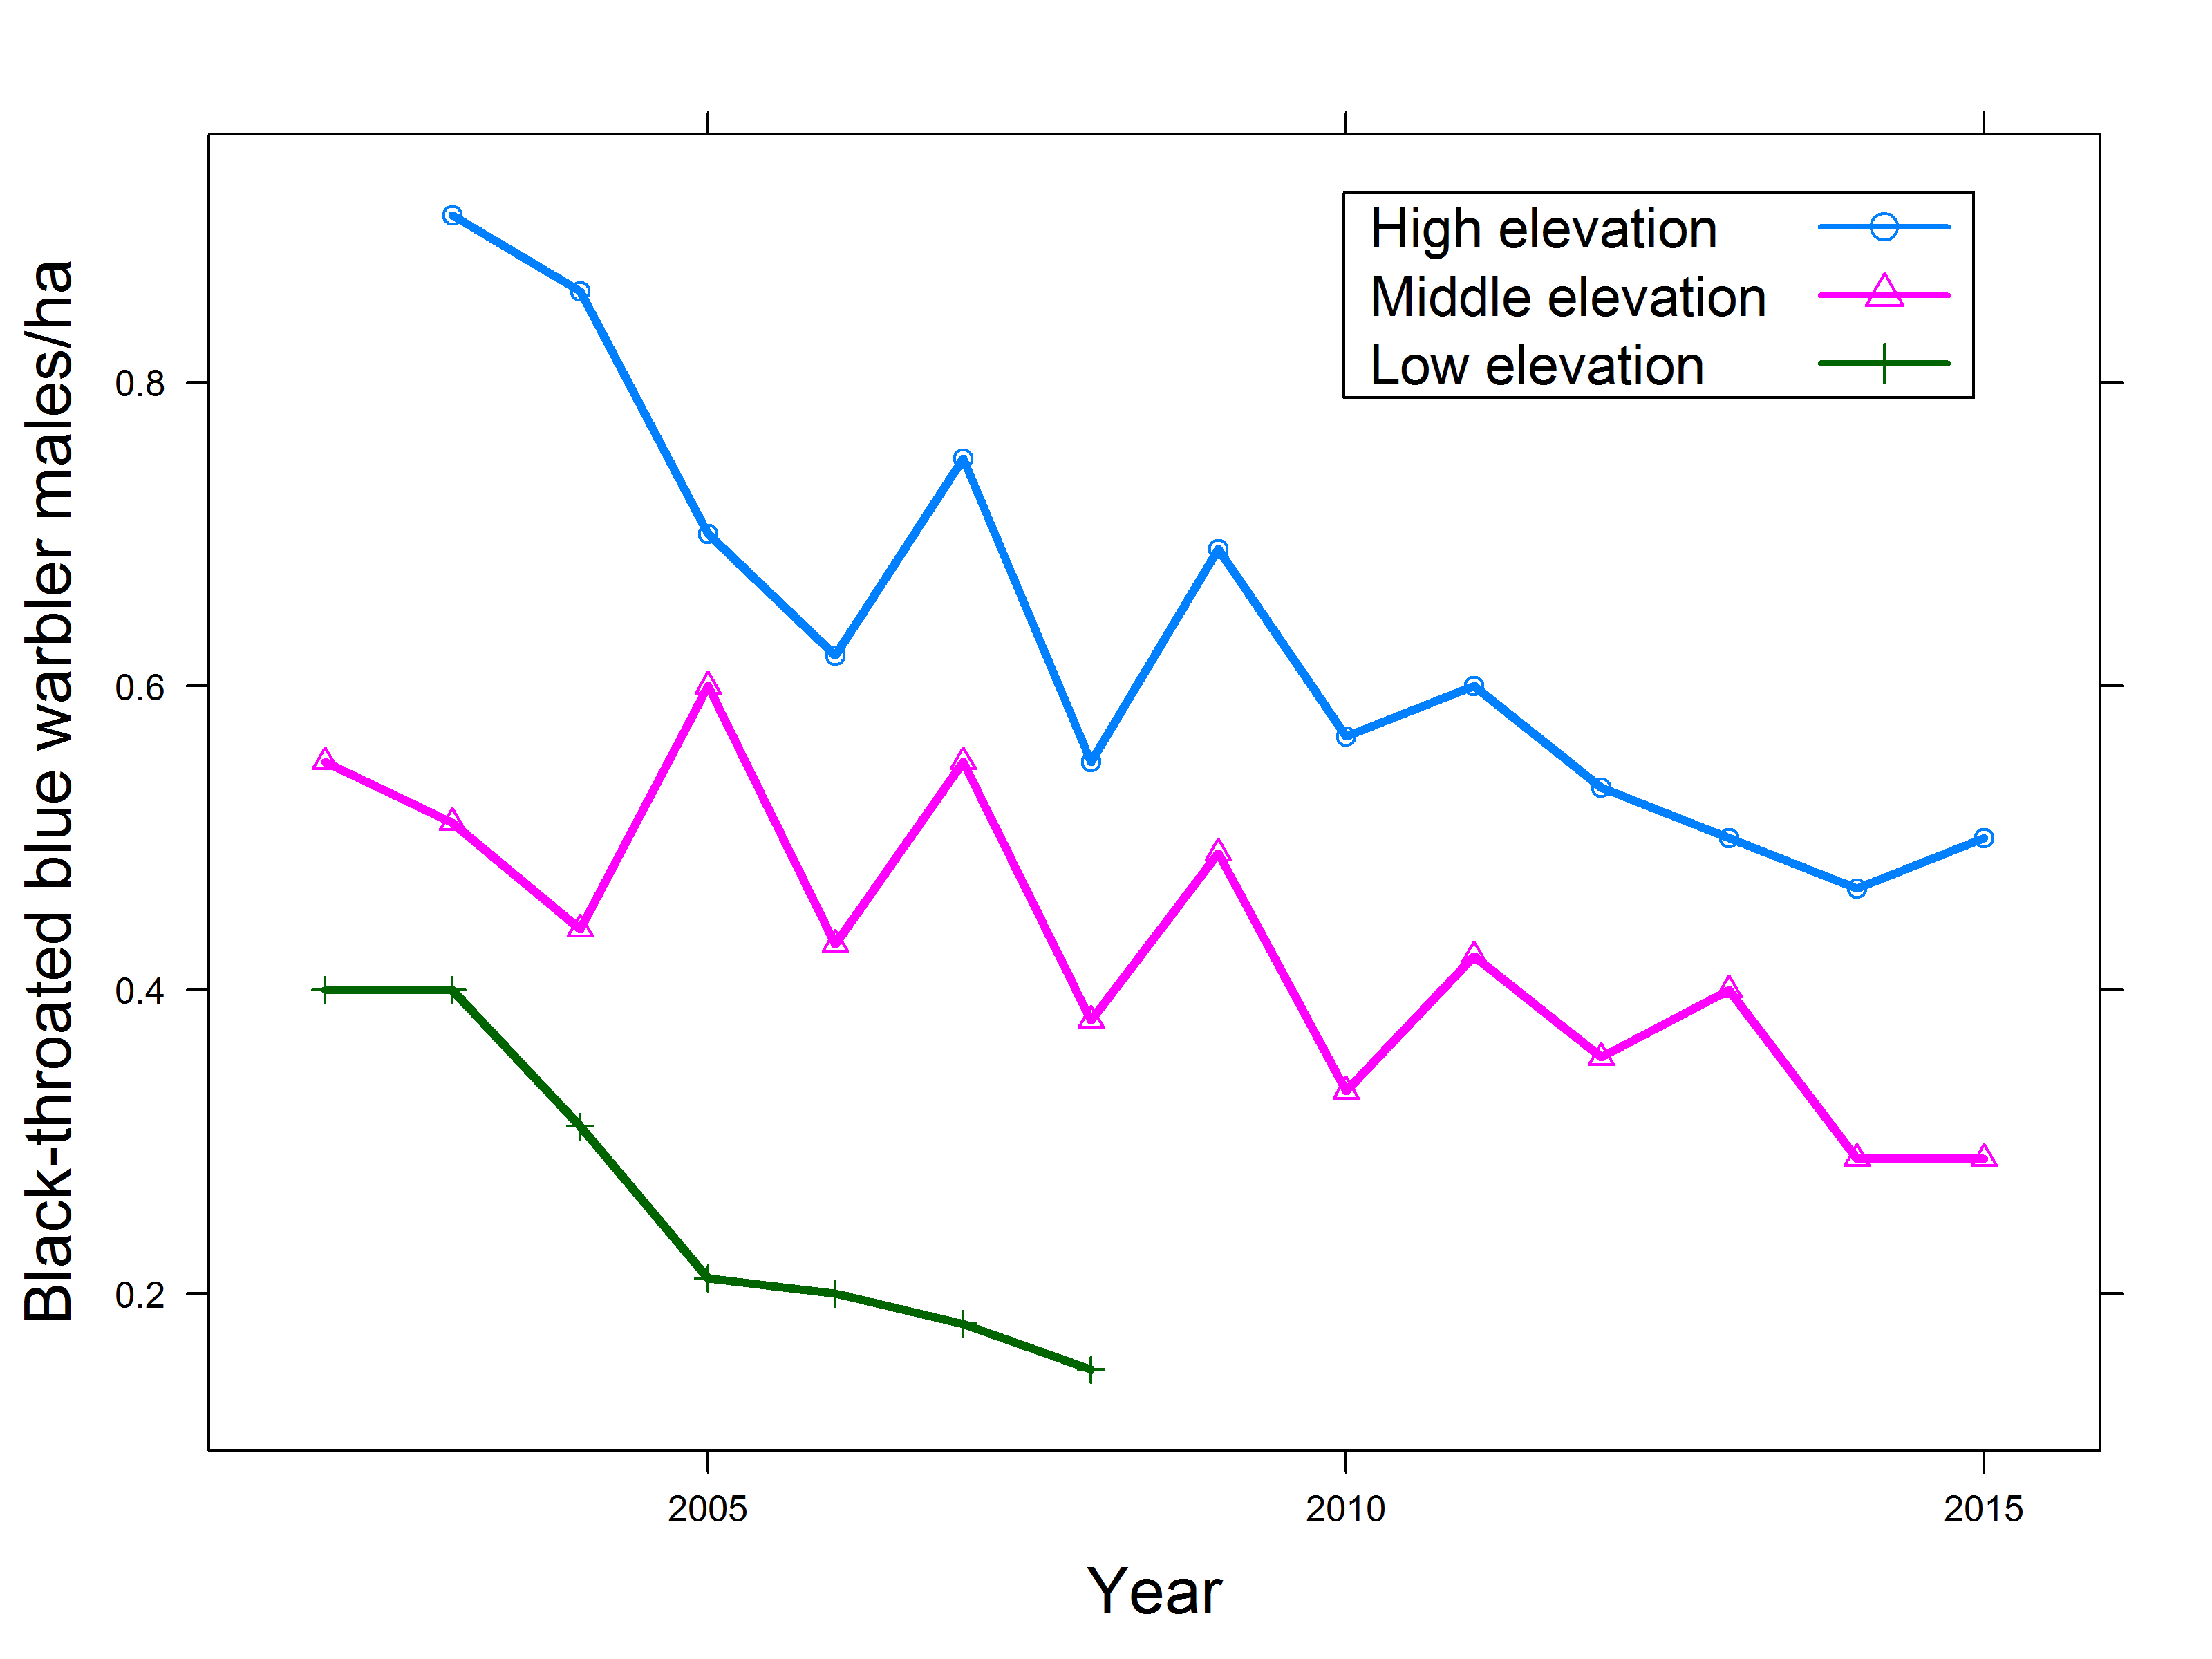
\includegraphics[width=0.8\textwidth]{figs/blue_density3plots}\let\thefootnote\relax\footnote{\tiny Data courtesy of Dr. RJ Cooper} \\ 
  Why are dynamics so different in the southern part of
  the range? \\
\end{frame}





\begin{frame}
  \frametitle{Example III -- Chiricahua Leopard Frog}
  \begin{columns}
    \begin{column}{0.5\textwidth}
      \fbox{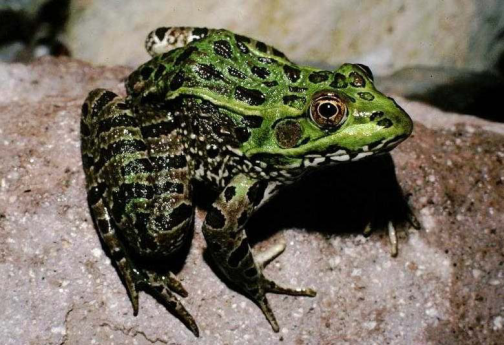
\includegraphics[width=\textwidth]{figs/lich}}
    \end{column}
    \begin{column}{0.5\textwidth}
      \fbox{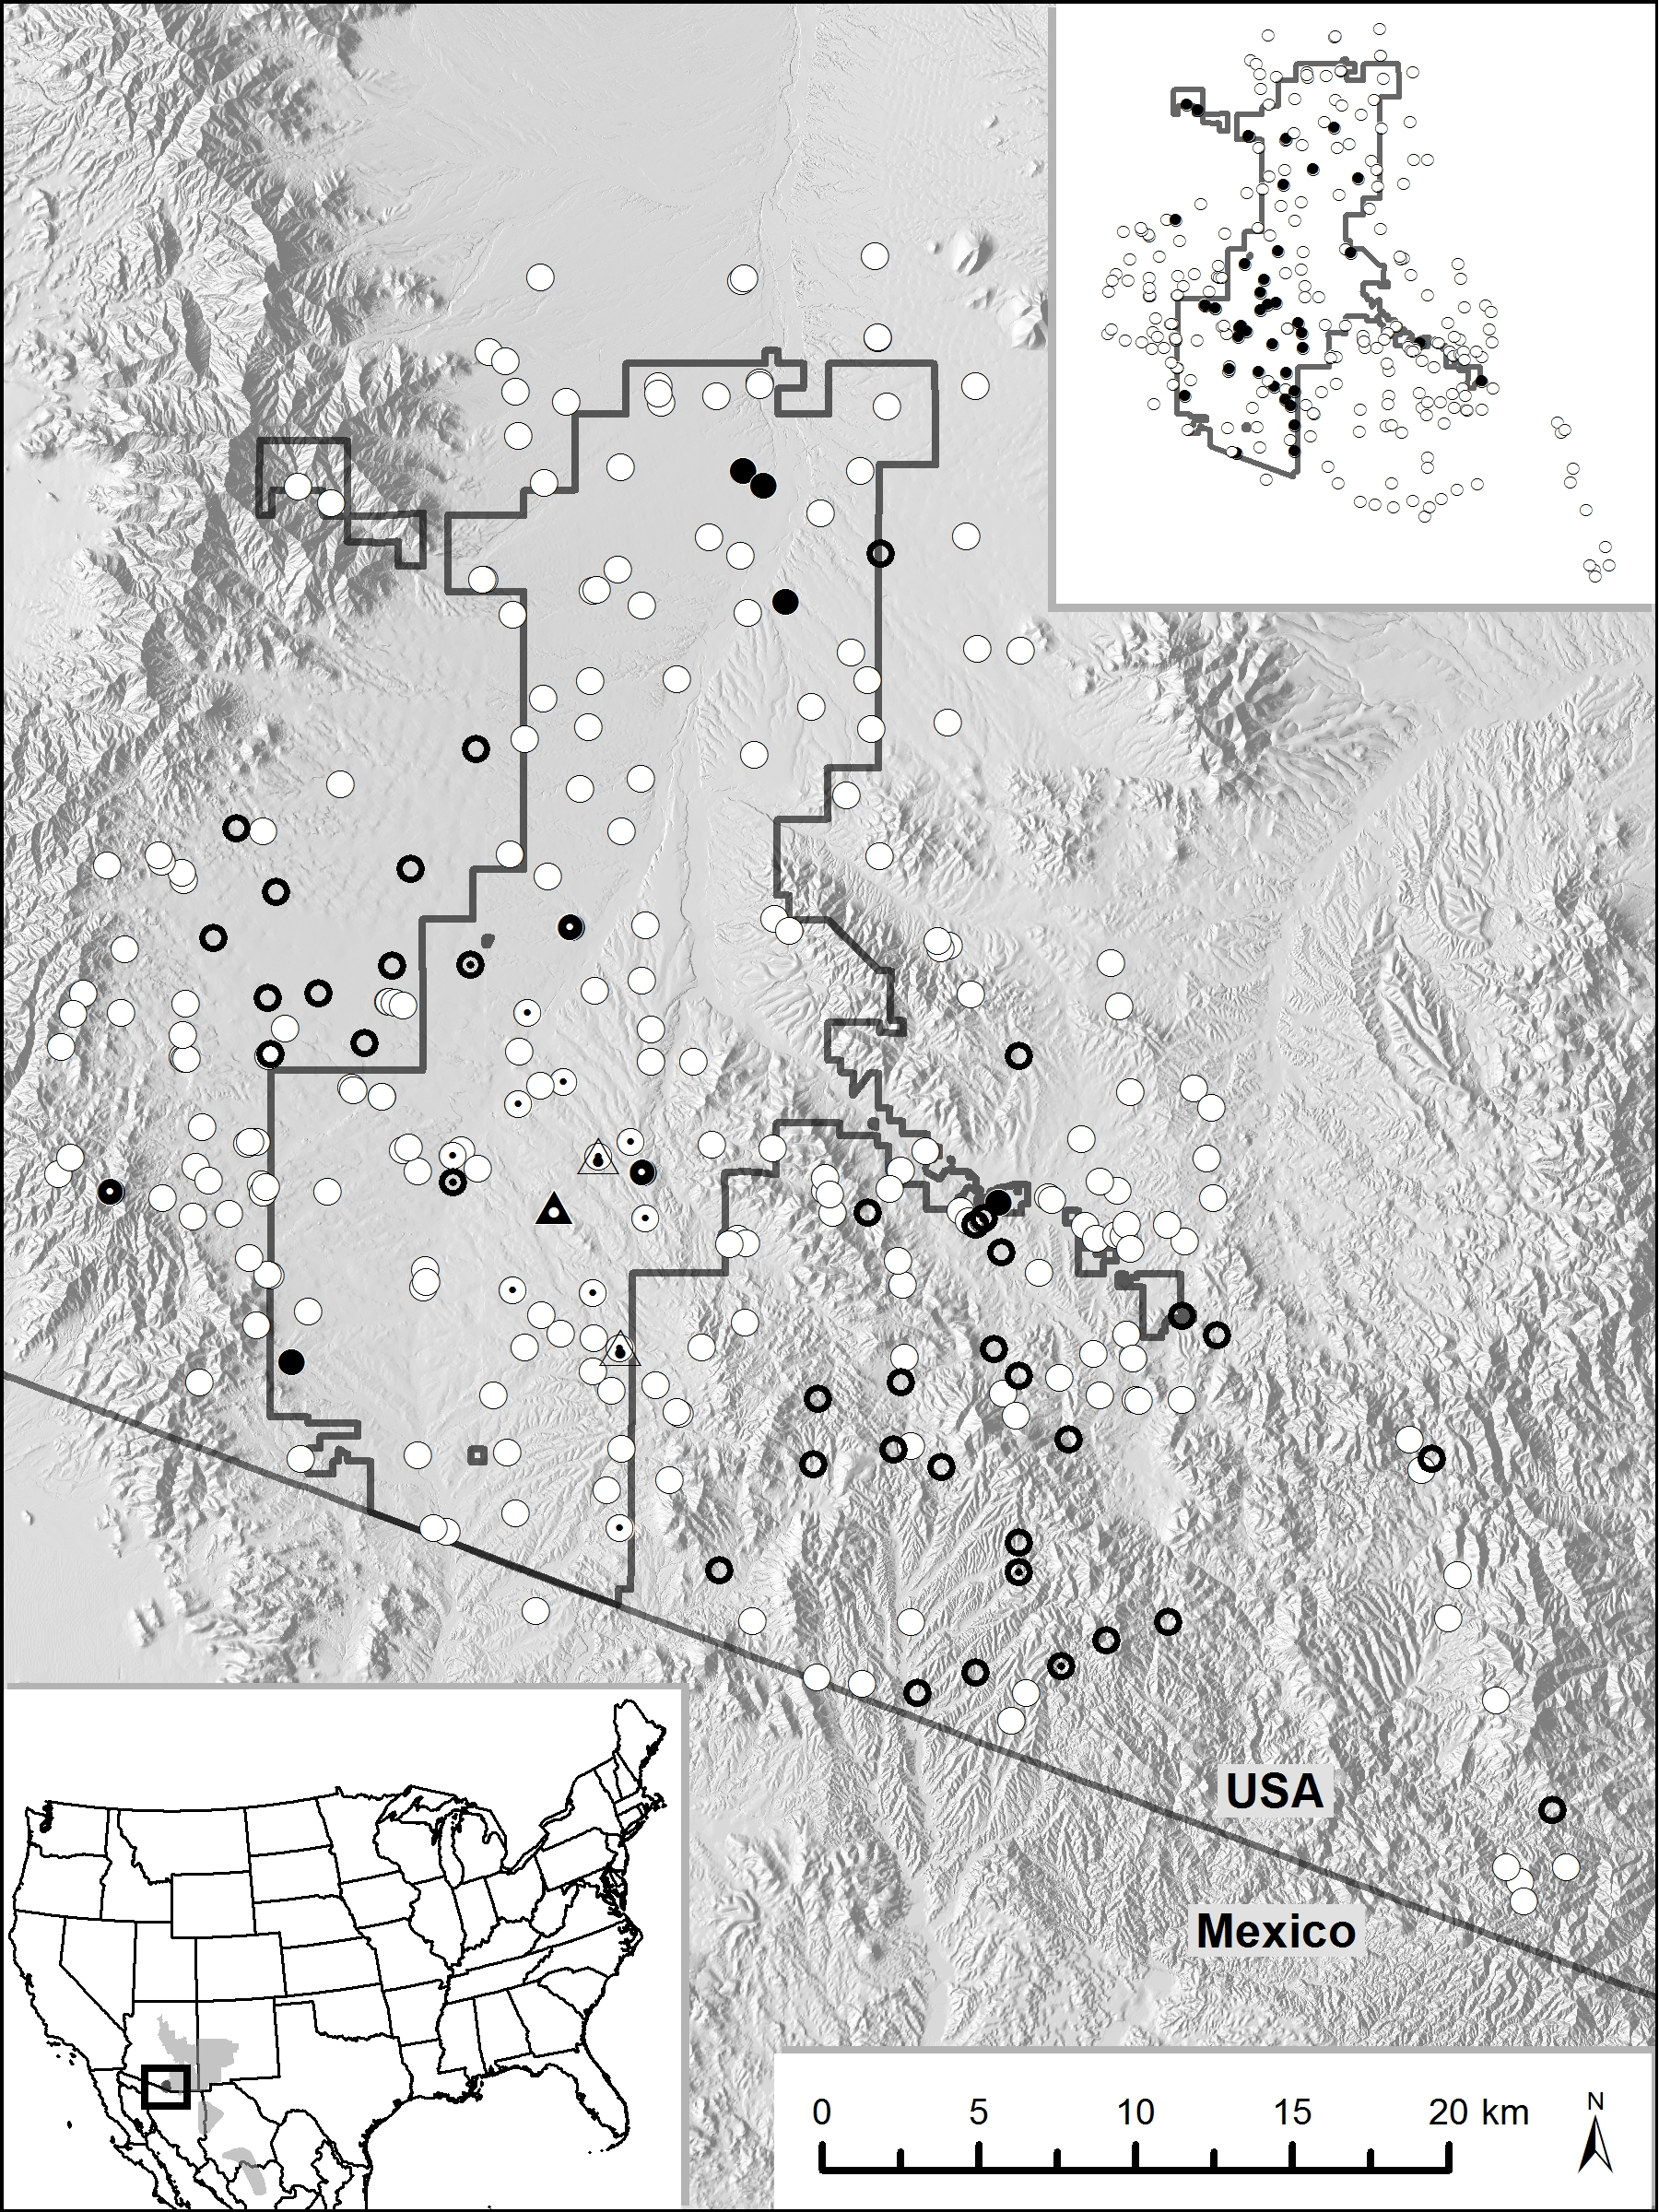
\includegraphics[width=\textwidth]{figs/lich-dist}}
    \end{column}
  \end{columns}
\end{frame}




\begin{frame}
  \frametitle{Recovery Plan}
  \begin{center}
    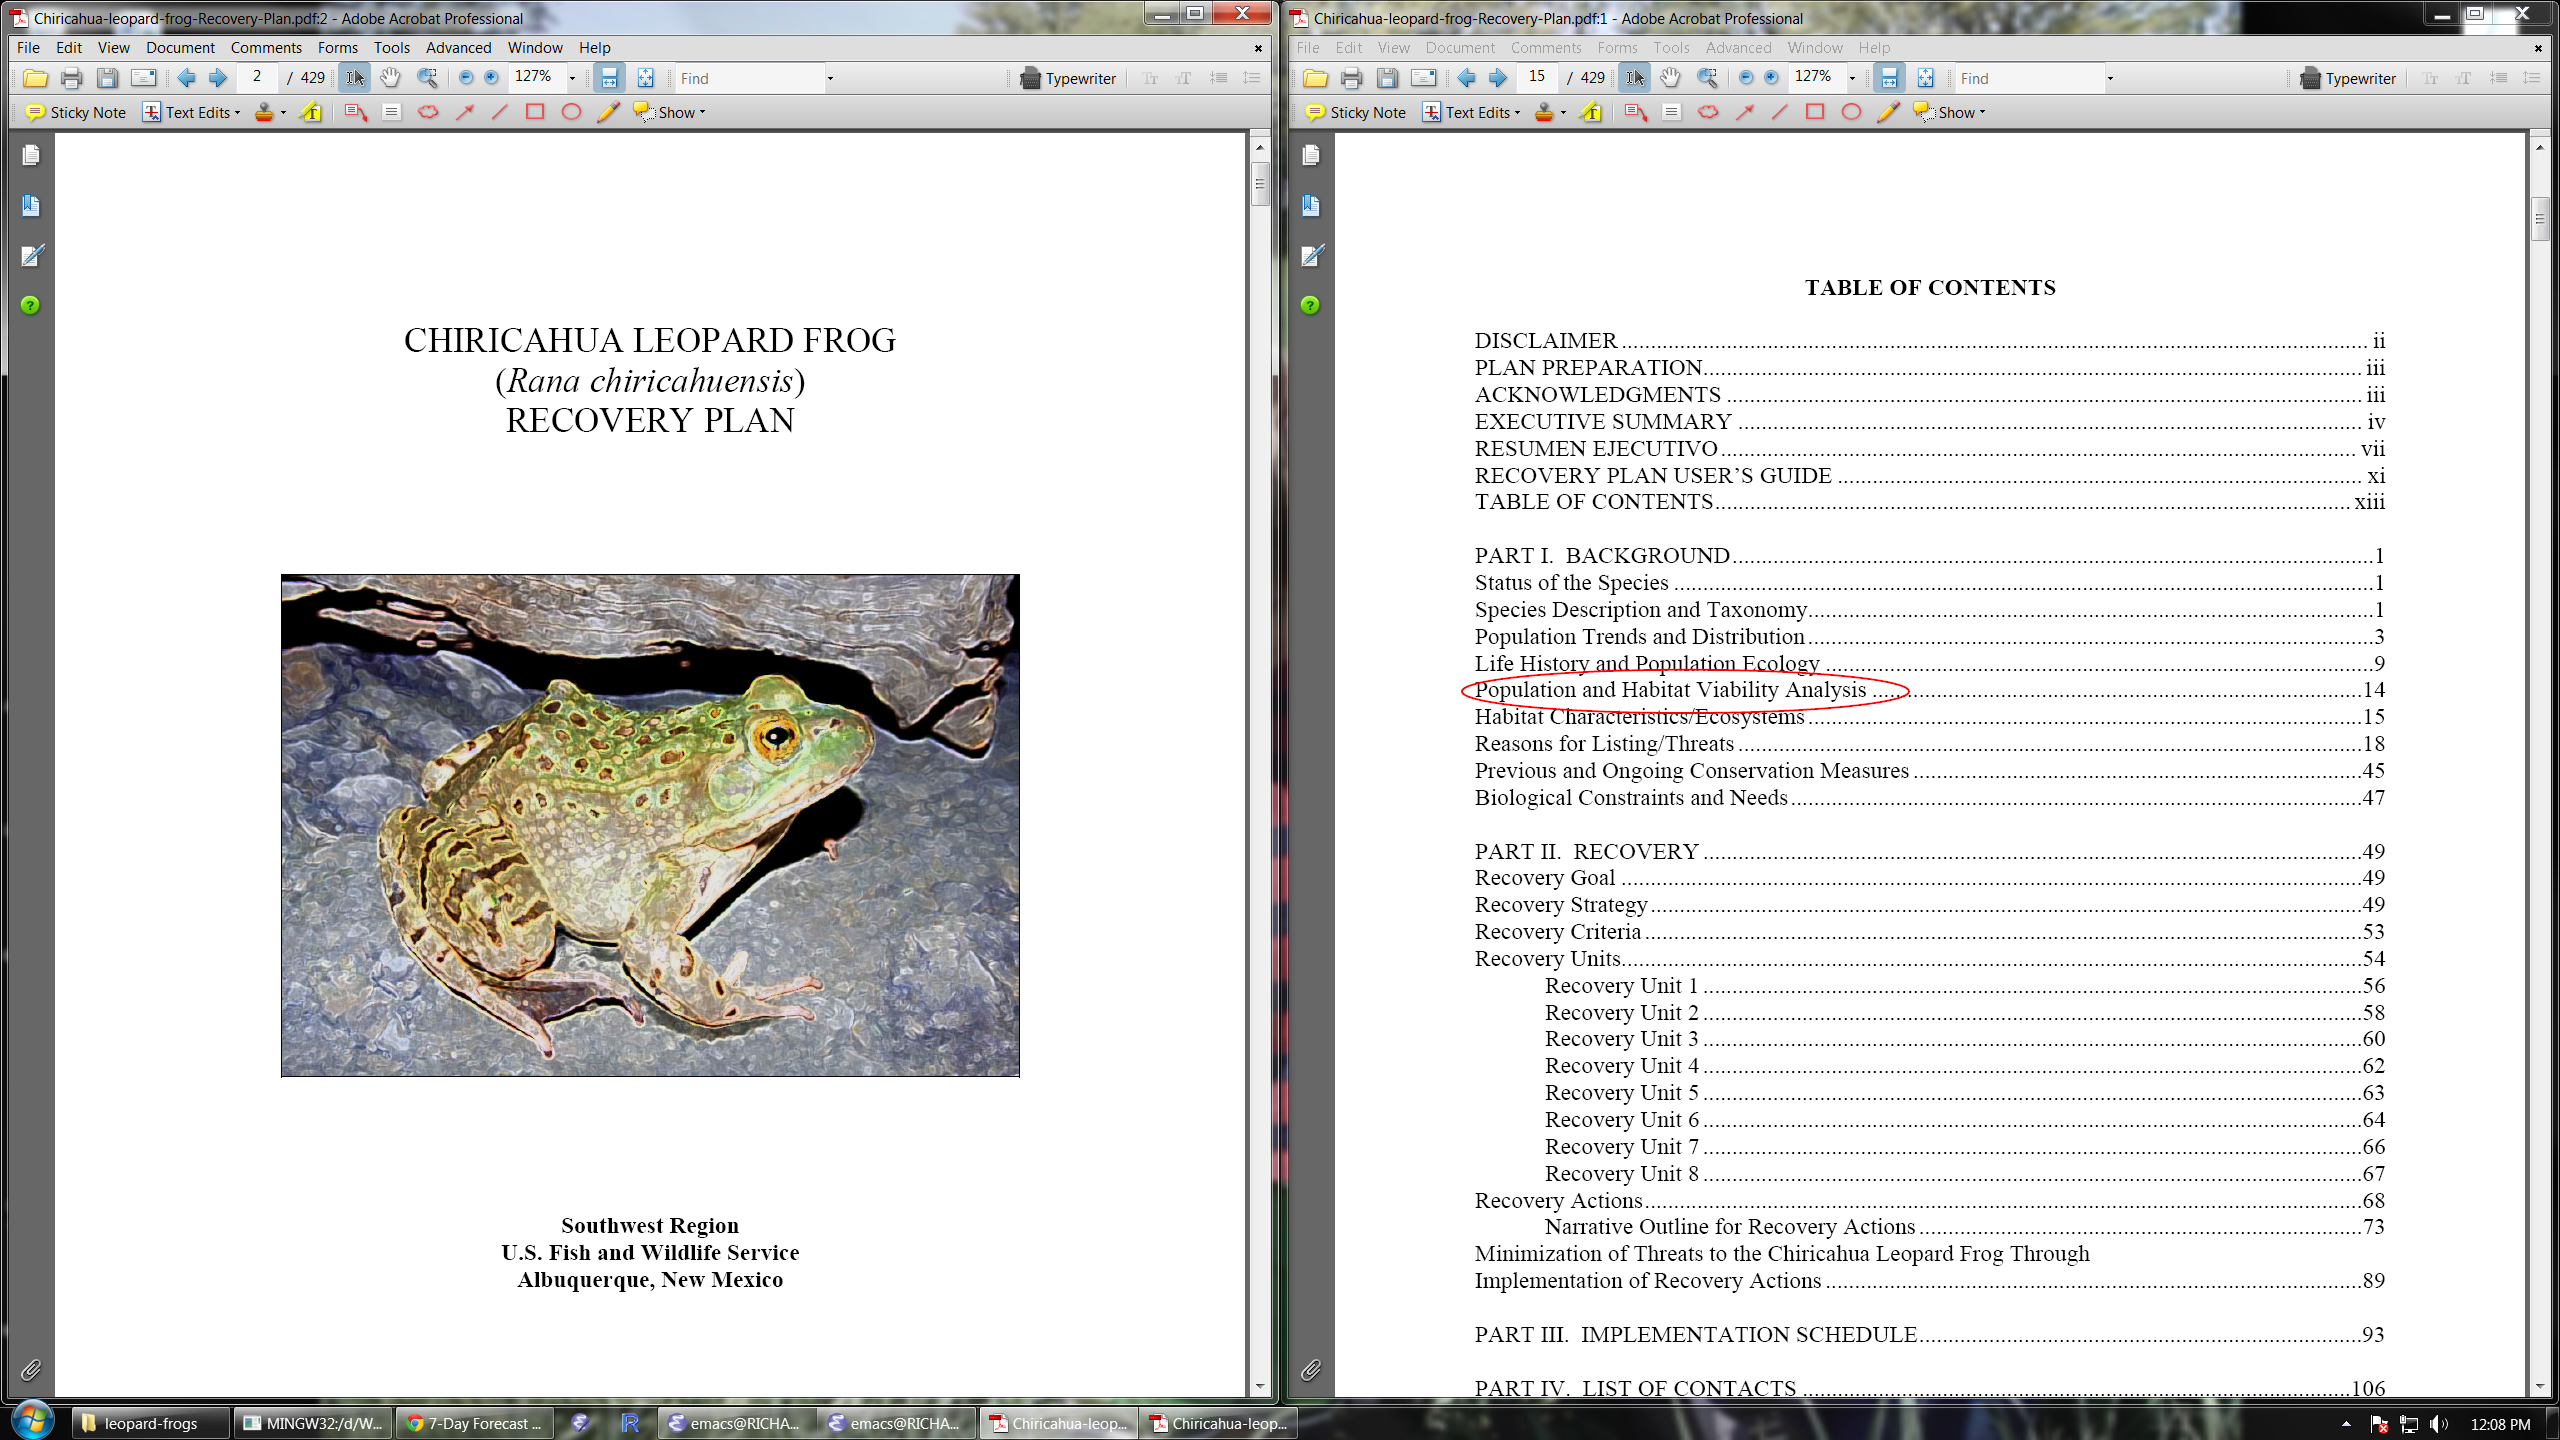
\includegraphics[width=\textwidth]{figs/lich-recovery-plan}
  \end{center}
\end{frame}



\begin{frame}
  \frametitle{Estimated extinction risk}
  % \begin{columns}
  %   \begin{column}{0.6\textwidth}
    %\begin{itemize}%[<+->]
      % \item<1-> We estimated extinction probability to be 2\% by 2100
      % \item[]
      % \item<1->
   Management options %What can be done about it?
        \begin{itemize}
          \item<1-> Control predators
          \item<1-> Increase hydroperiod in existing wetlands
          \item<1-> Create new wetlands\dots
%        \item<6-> \dots but where?
        \end{itemize}
        % \item<2->
    \pause
    \vfill
    Extinction risk was predicted to be 4\% after 50
    years. Restoring just 1 pond, reduced the risk to 2.5\%.  \\
%    \end{itemize}
    % \pause
    % \vfill
    \centering
    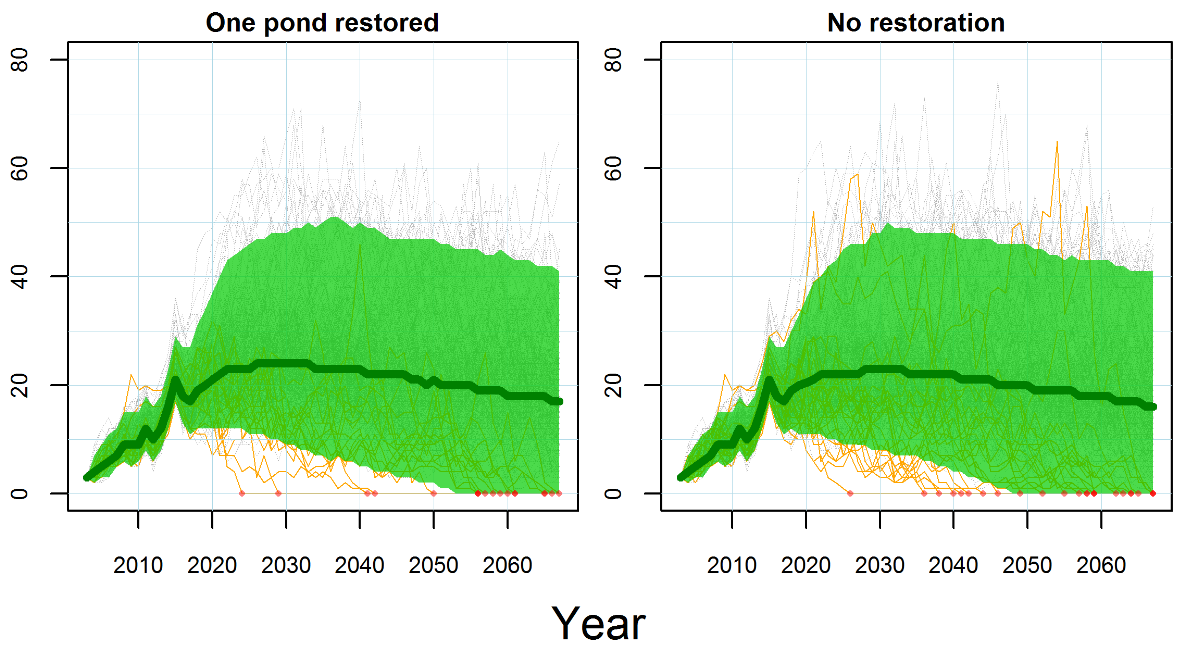
\includegraphics[width=0.7\textwidth]{figs/lich-forecasts}
%     \end{column}
%     \begin{column}{0.4\textwidth}
%       \begin{center}
% %        \includegraphics[width=0.4\textwidth]{figs/extinction3}
%         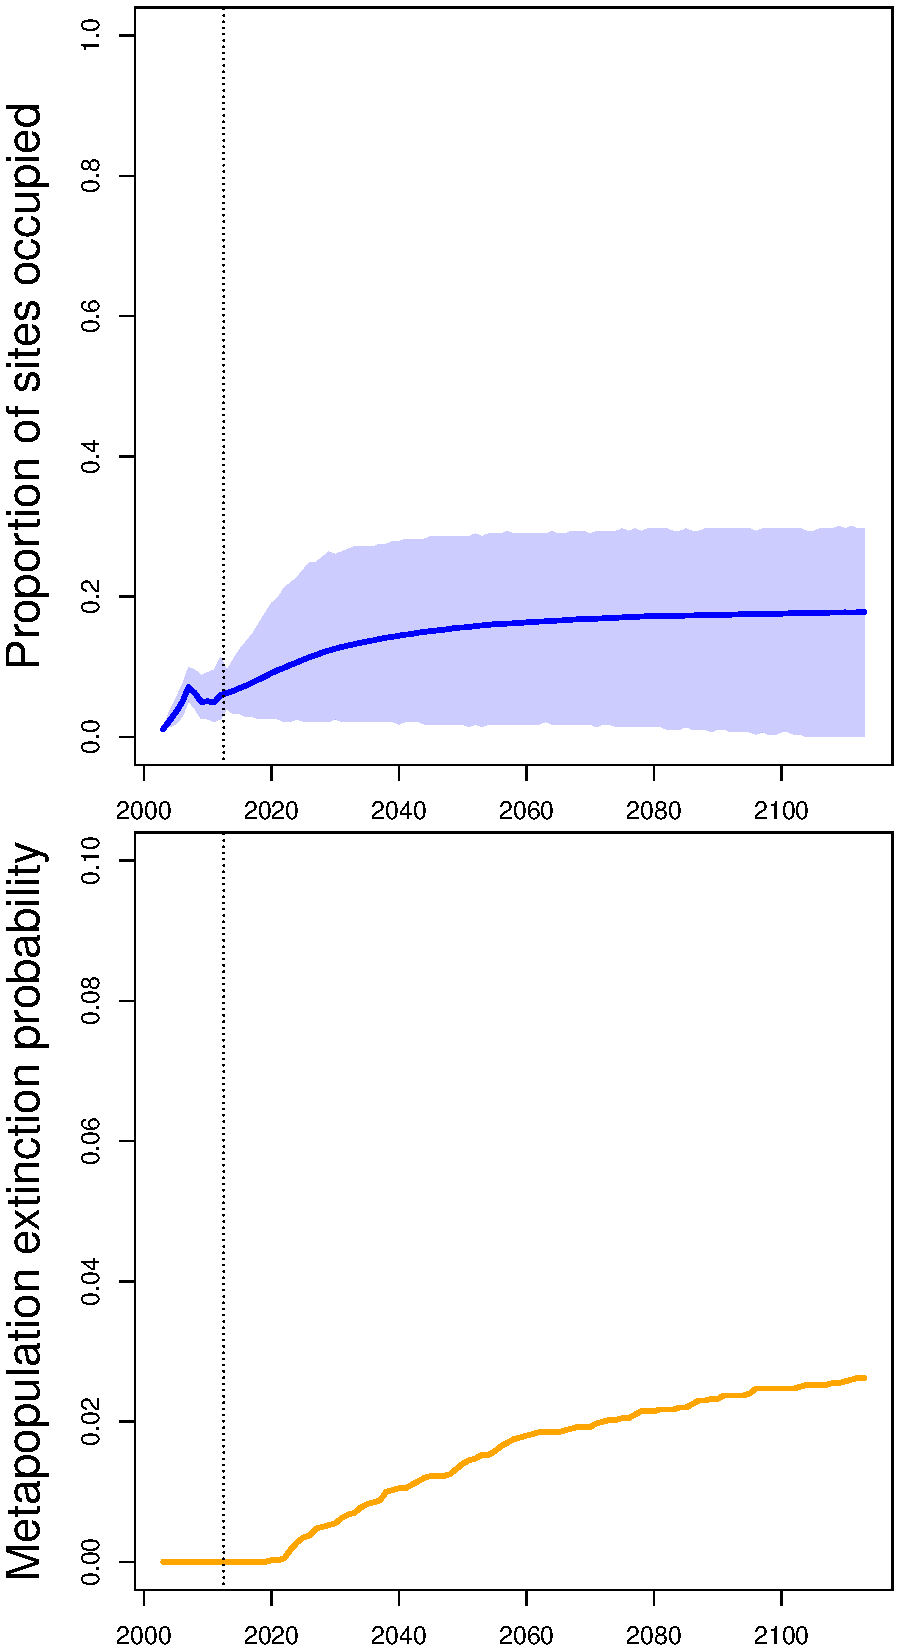
\includegraphics[width=\textwidth]{figs/proj-ext-JAPPL}
%       \end{center}
%     \end{column}
%   \end{columns}
\end{frame}



% \begin{frame}
%   \frametitle{Extinction risk}
%   \begin{center}
%     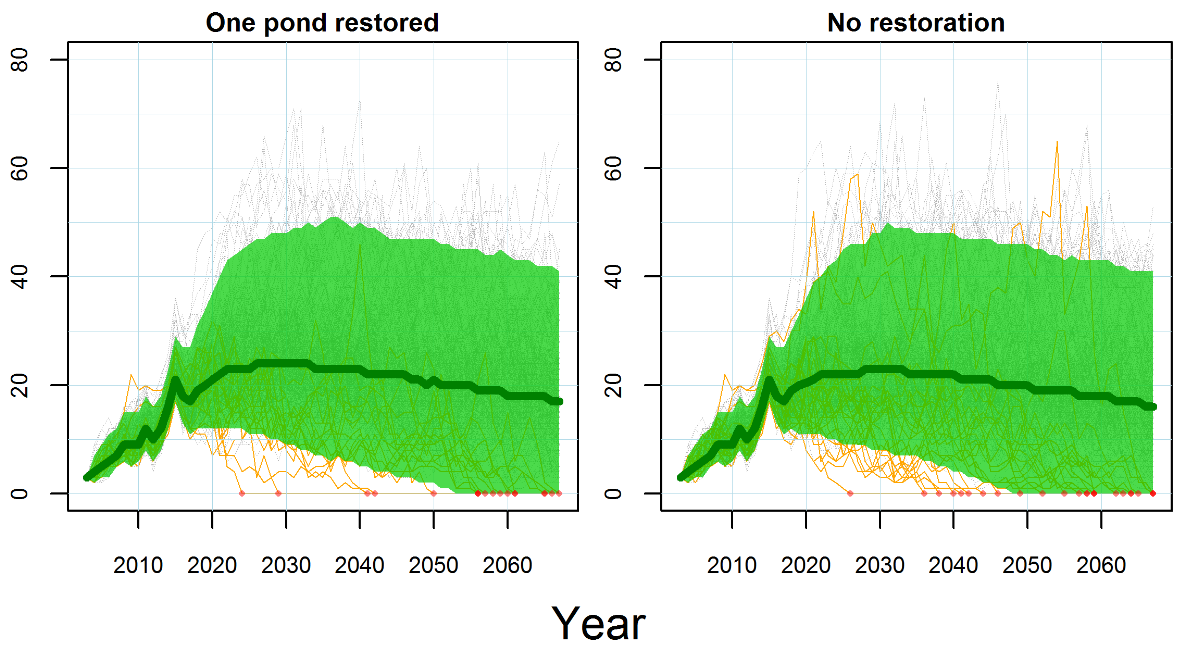
\includegraphics[width=\textwidth]{figs/lich-forecasts}
%   \end{center}
% \end{frame}



\begin{frame}{Embedded Animation}
  \frametitle{Colonization Probability Maps}
  \centering
%  \begin{center}
%%     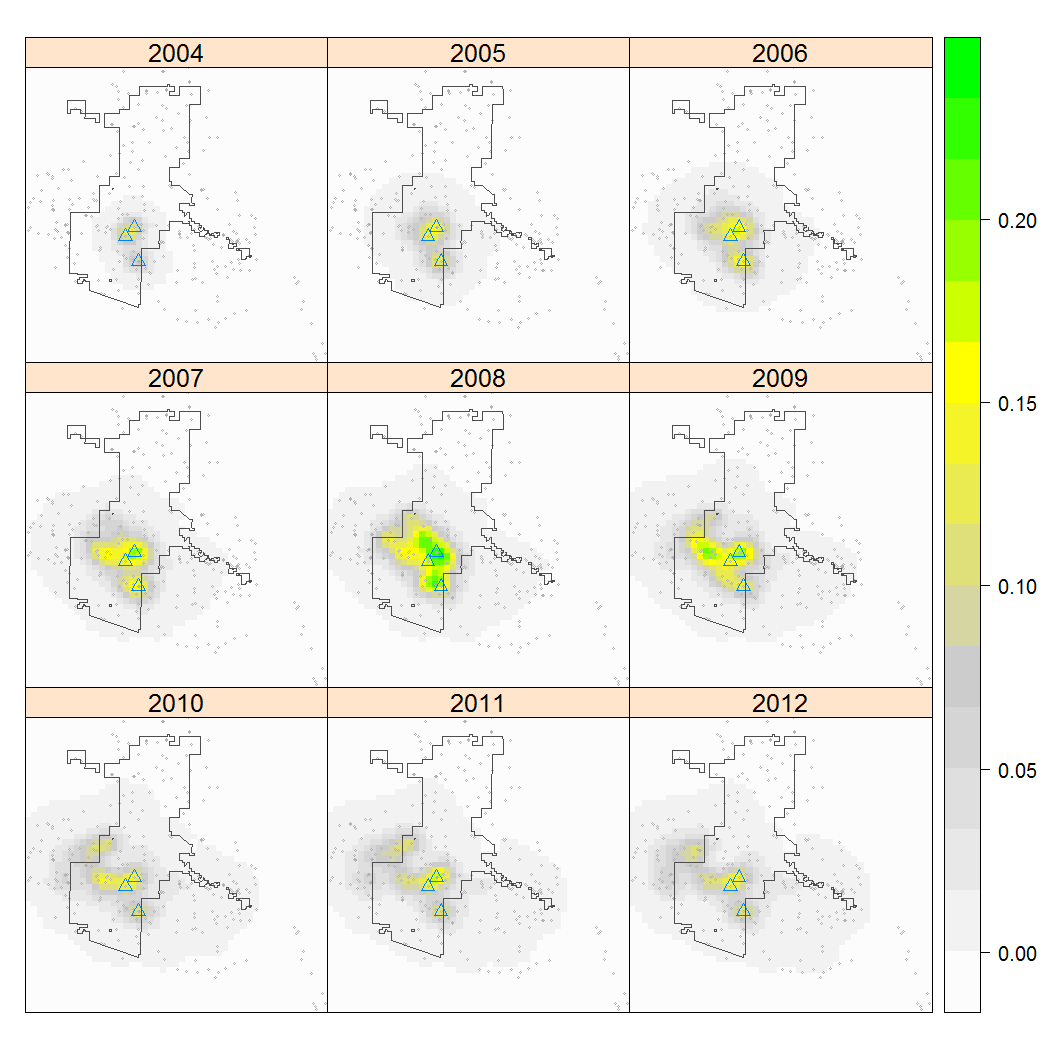
\includegraphics[width=0.7\textwidth]{figs/colMap1-9nohill} \\
% \end{center}
% \includegraphics[width=0.7\textwidth]{figs/colMap-animation2} \\
%% \animategraphics[loop,width=0.7\textwidth]{2}{figs/colMap}{2004}{2012} \\
  \transduration<0-8>{1}
  \multiinclude[<+->][format=png,graphics={width=0.7\textwidth}]{figs/colMap} \\
\end{frame}




\begin{frame}
  \frametitle{Example IV -- South Florida Deer Study}
  \large
  {\bf Objectives}
  \begin{enumerate}[\bf 1.]
    \item Understand effects of hydrology, hunting, and predation on
    deer population dynamics 
    \item<1-> Develop a camera trapping study for large-scale
    investigation and monitoring of deer populations
  \end{enumerate}
  \vfill
  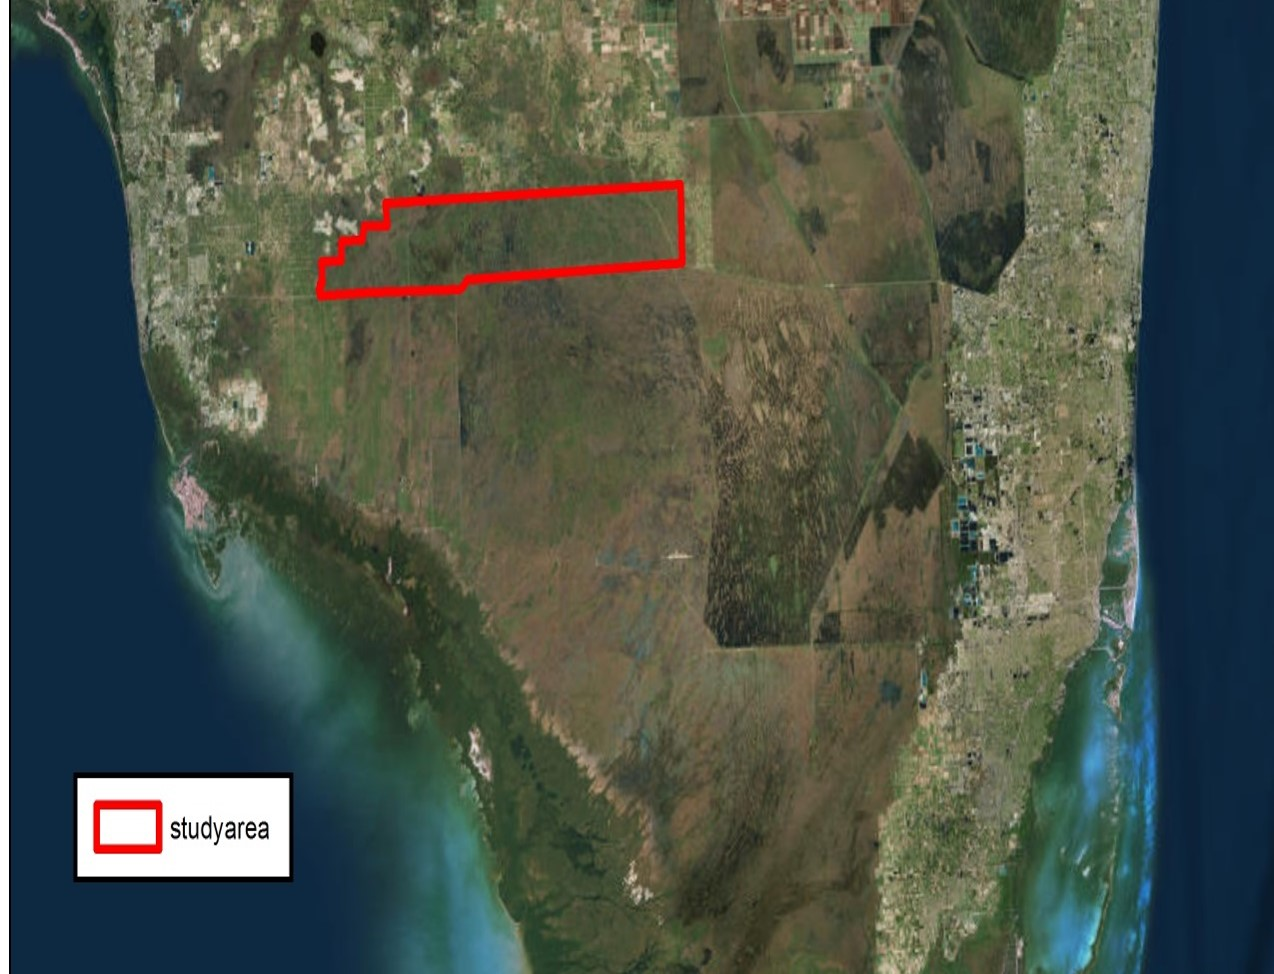
\includegraphics[width=0.49\textwidth,trim = 0mm 8mm 0mm 0mm, clip]{figs/studyArea} \hfill
  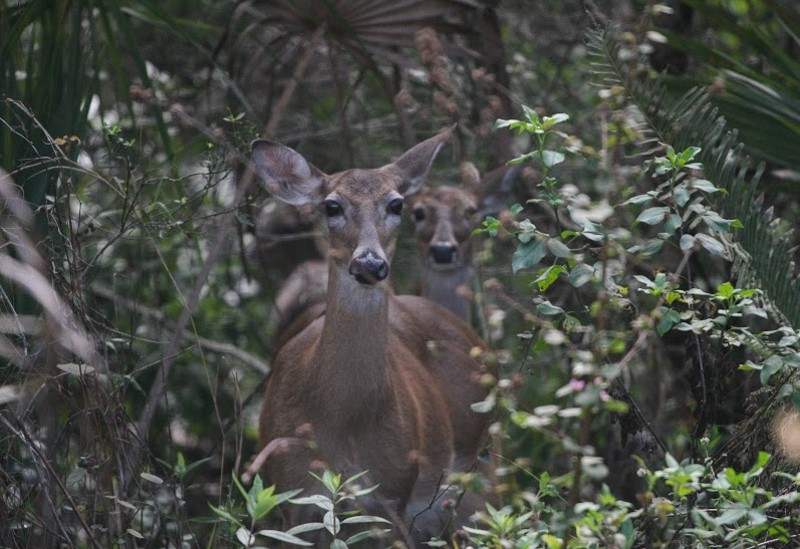
\includegraphics[width=0.49\textwidth]{figs/deer2}
\end{frame}





\begin{frame}
  \frametitle{Camera study}
  \centering
  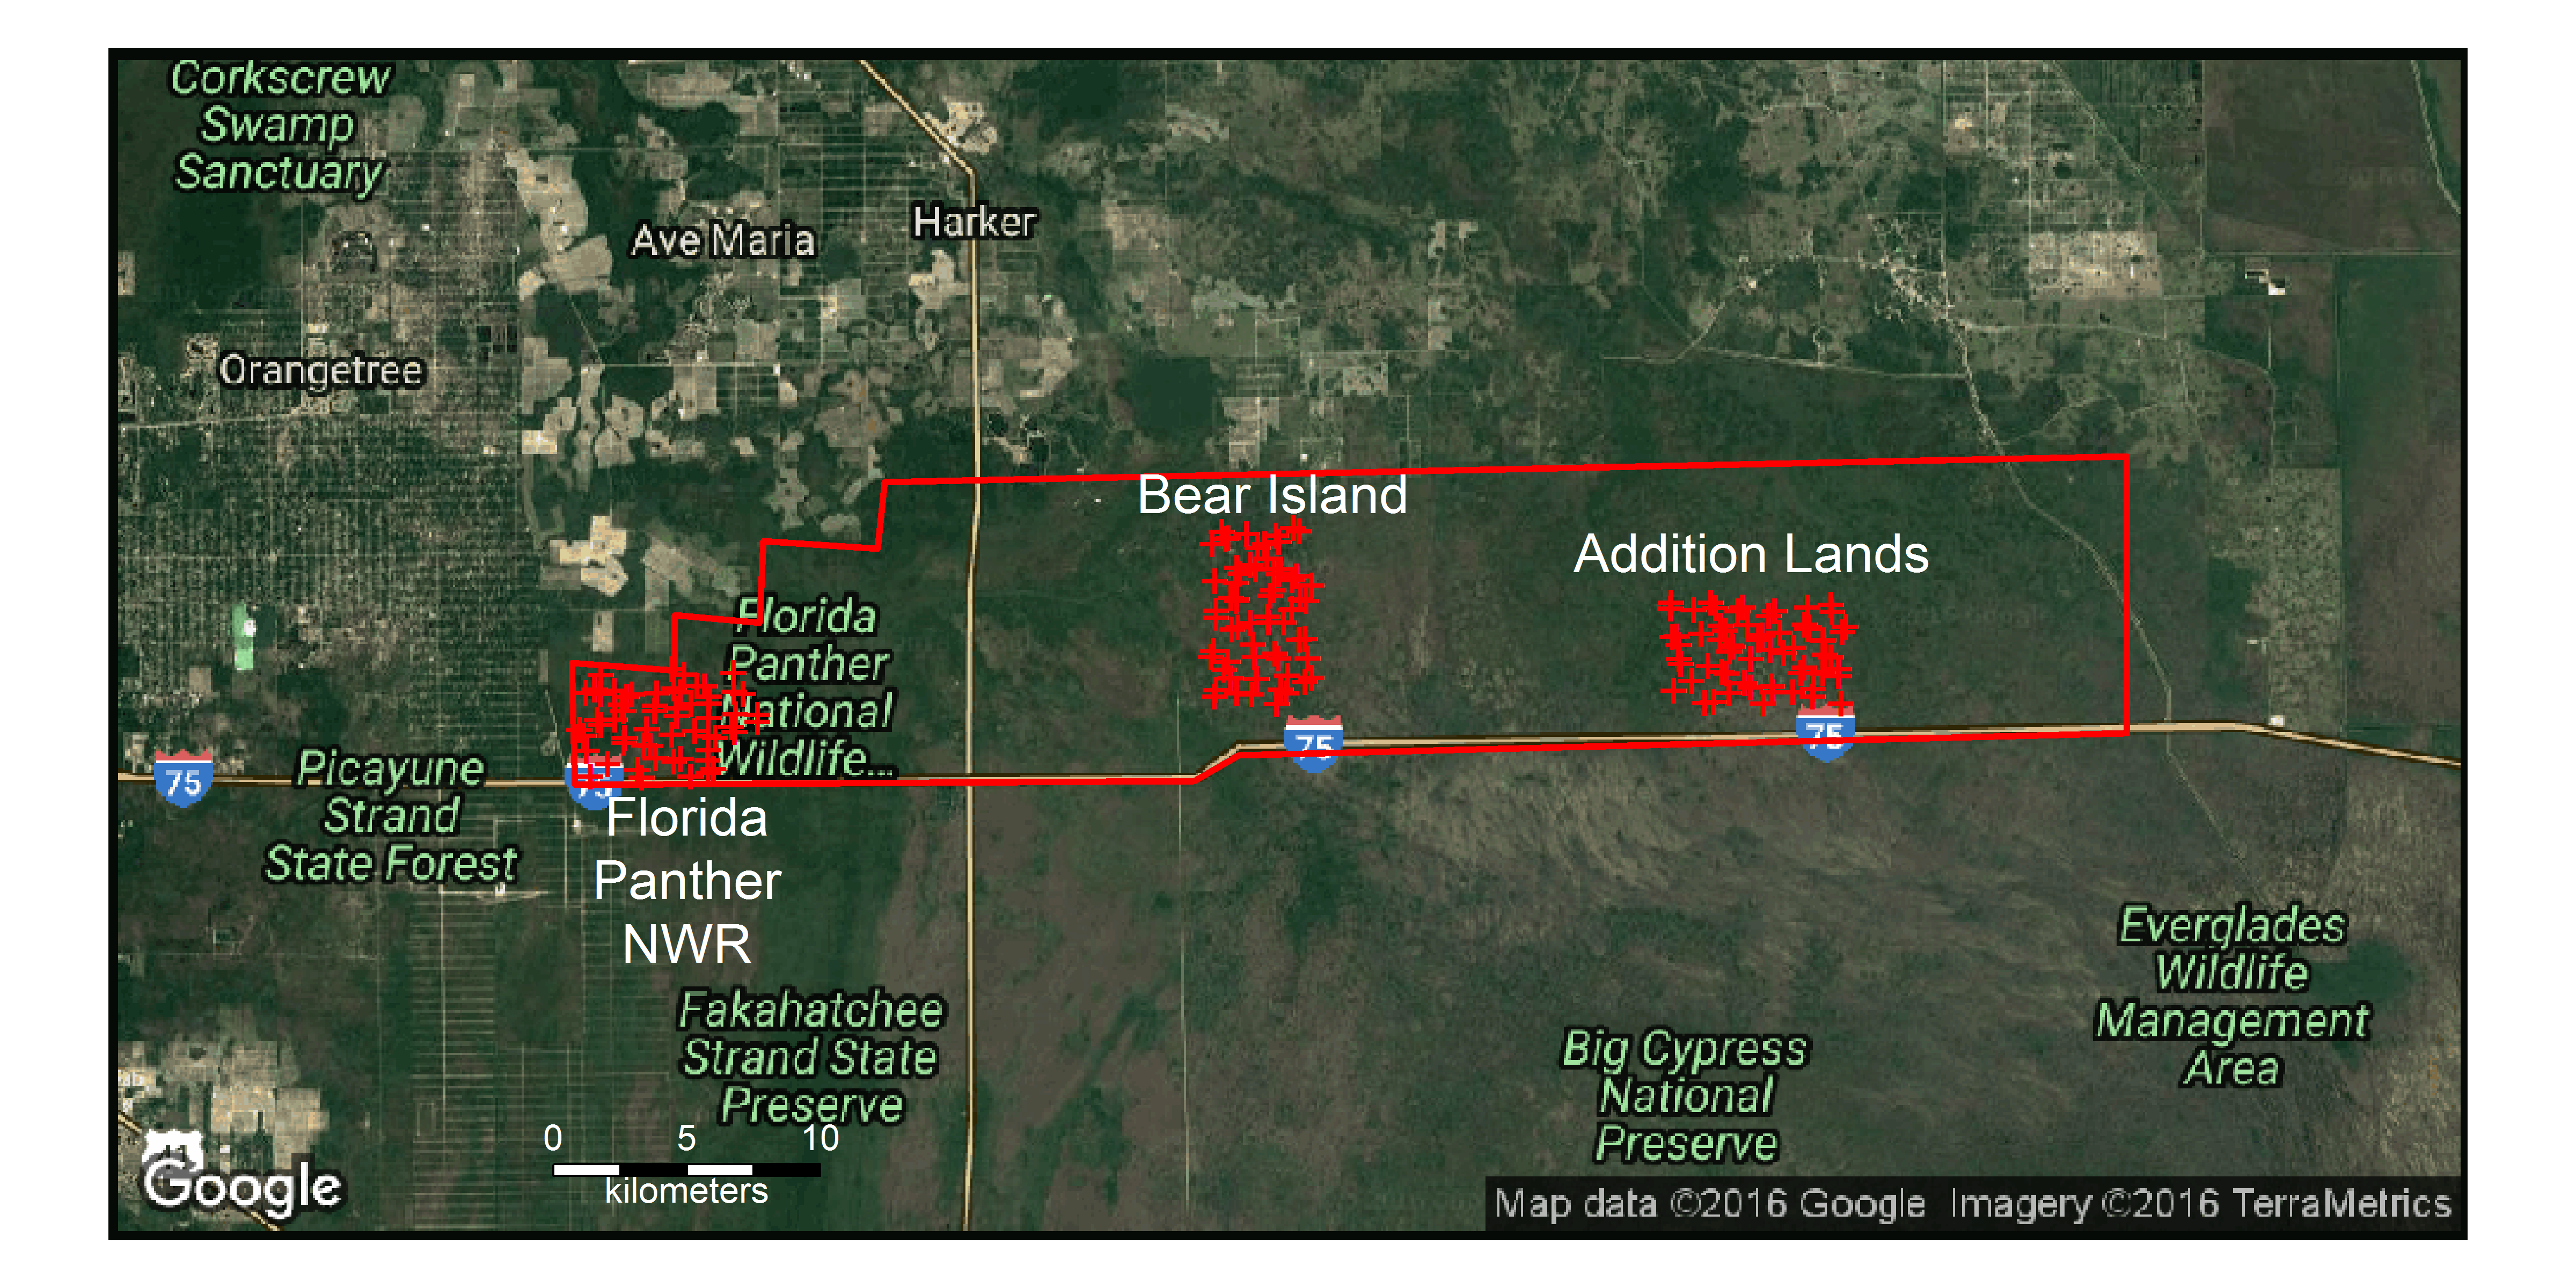
\includegraphics[width=\textwidth]{figs/FL-base-cameras} \\
  \vfill
  \begin{columns}
    \begin{column}{0.05\textwidth}
    \end{column}
    \begin{column}{0.35\textwidth}
      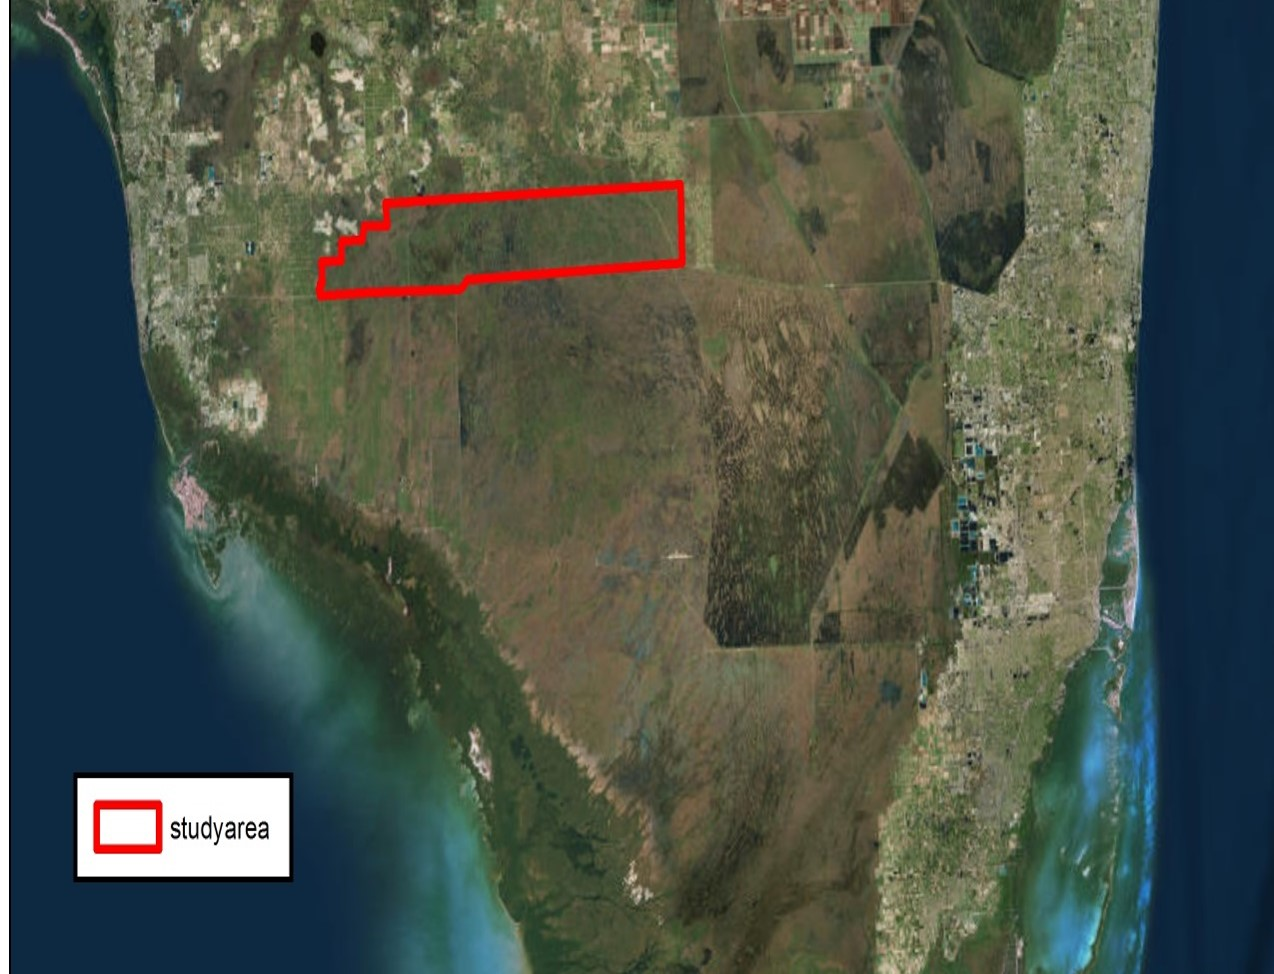
\includegraphics[width=\textwidth,trim = 0mm 8mm 0mm 0mm, clip]{figs/studyArea}
    \end{column}
    \begin{column}{0.6\textwidth}
      \small
      \begin{itemize}
        \item 180 cameras
        \item Operated Jan 2015 -- Jan 2018
        \item Spanning hunting and hydrology gradients
      \end{itemize}
    \end{column}
  \end{columns}
\end{frame}




\begin{frame}
  \frametitle{Telemetry data}
  \centering
  \bf
  $>$250 deer collared since January 2015 \\
  \begin{columns}
    \column{\dimexpr\paperwidth-10pt}
    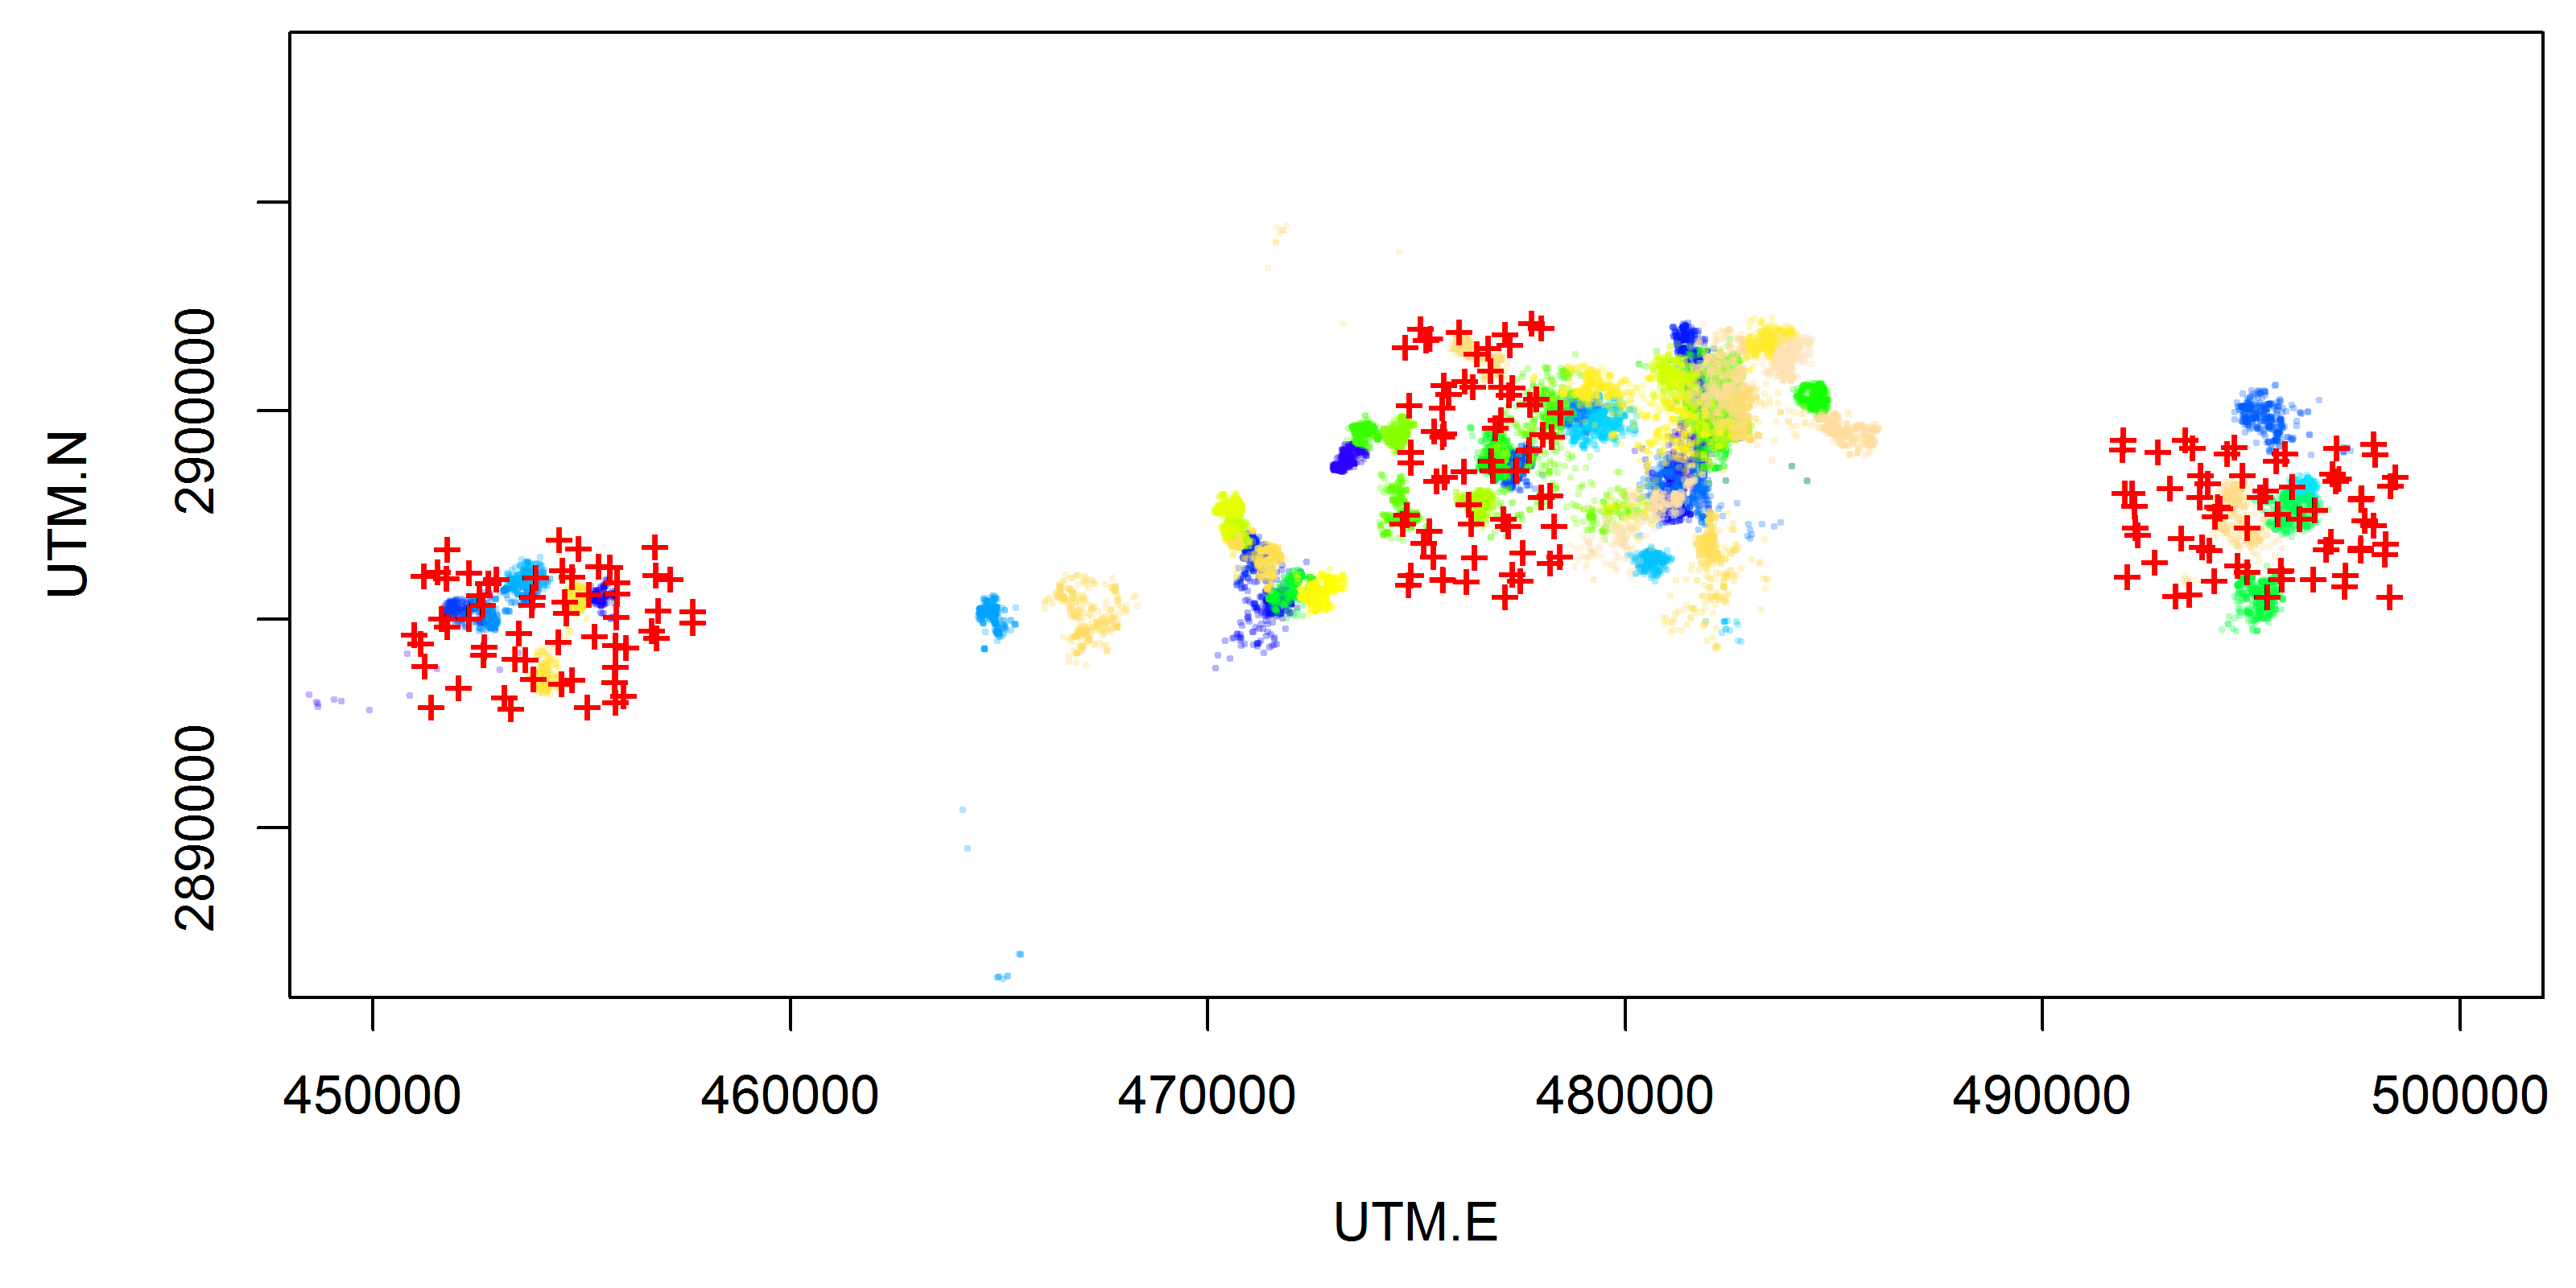
\includegraphics[width=\textwidth]{figs/camTelem}
  \end{columns}
\end{frame}



\begin{frame}
  \frametitle{Abundance over time}
  \centering
  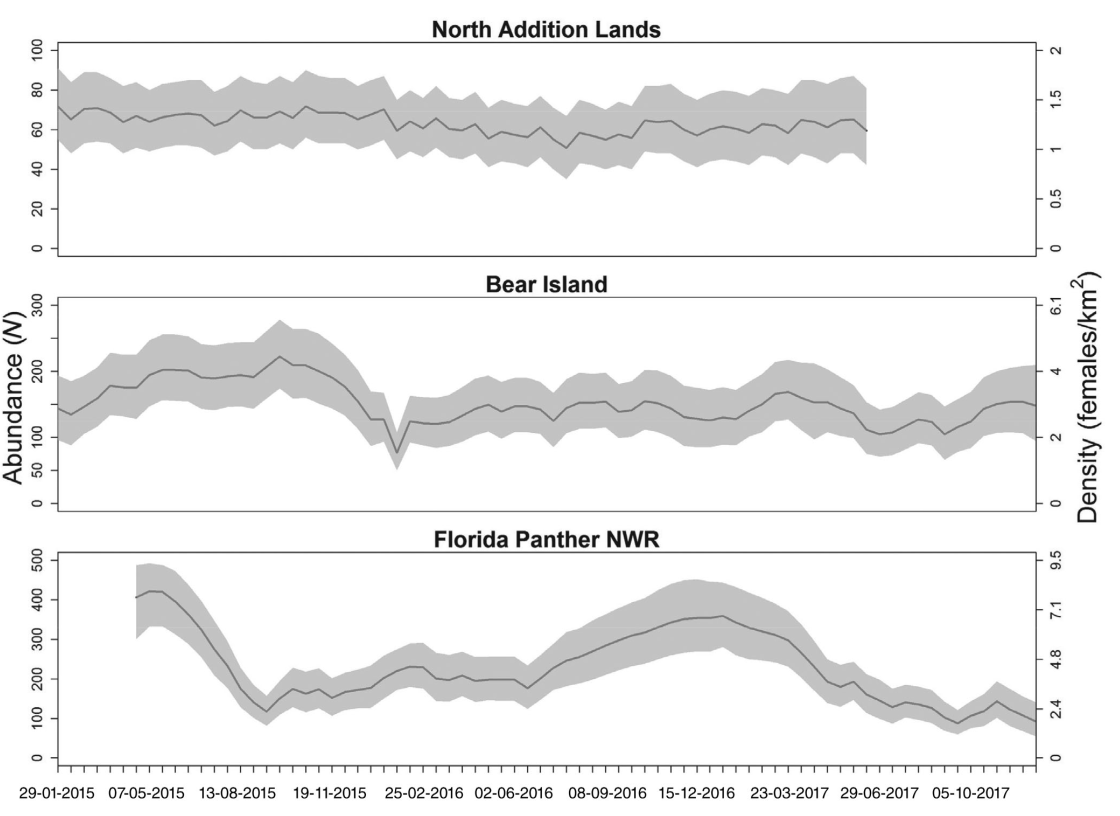
\includegraphics[width=0.9\textwidth]{figs/deer-N-timeseries} \\
\end{frame}




\begin{frame}
  \frametitle{Survival and predation rate}
  \centering
  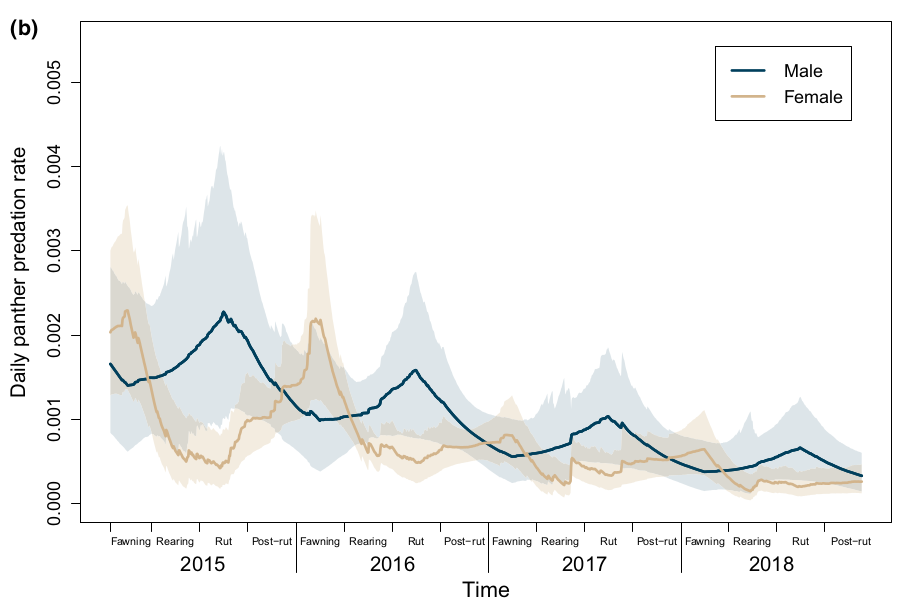
\includegraphics[width=0.95\textwidth]{figs/deer-pred-time} \\
\end{frame}



\section{Assignment}


\begin{frame}
  \frametitle{Assignment}
  \begin{columns}
    \begin{column}{0.6\textwidth}
      \large
      \begin{enumerate}[\bf 1.]
        \item<1-> Read Chapters 1 and 2 of Conroy and Carroll
        \item[]
        \item<1-> Complete the introductory ``quiz'' found here: \\
          \tiny \url{https://goo.gl/forms/OpmugP5lmMrrXTIY2}
      \end{enumerate}
    \end{column}
    \begin{column}{0.4\textwidth}
      \fbox{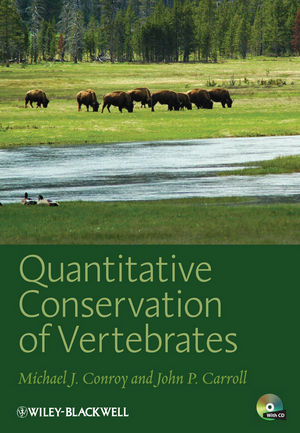
\includegraphics[width=\textwidth]{figs/Conroy_Carroll}}
    \end{column}
  \end{columns}
\end{frame}




\begin{frame}
  \frametitle{Tips for success in this course}
  \begin{enumerate}[(1)]
    \large
    \item Take notes on the handouts 
      % \pause \vfill
    \item[]
    \item Review notes before each lecture 
%    \pause \vfill
    \item[]
    \item Finish lab assignments during lab %\\
%    \pause \vfill
    \item[]
    \item Ask questions %\\
%    \pause \vfill
    \item[]
    \item Visit with me or the TAs during office hours %\\
%    \pause \vfill
  \end{enumerate}
\end{frame}



\section{Syllabus}




\begin{frame}
  \frametitle{Syllabus}
  \begin{columns}%[T]
    \begin{column}{0.5\textwidth}
      \fbox{\includegraphics[width=\textwidth]{../../APD-syllabus.pdf}}
    \end{column}
  \end{columns}
\end{frame}








\end{document}
